%%%%%%%%%%%%%%%%%%%%%%%%%%%%%%%%%%%%%%%%%%%%%%%%%%%%%%%%%%%%%%%%%%%%%
%%                                                                 %%
%% Please do not use \input{...} to include other tex files.       %%
%% Submit your LaTeX manuscript as one .tex document.              %%
%%                                                                 %%
%% All additional figures and files should be attached             %%
%% separately and not embedded in the \TeX\ document itself.       %%
%%                                                                 %%
%%%%%%%%%%%%%%%%%%%%%%%%%%%%%%%%%%%%%%%%%%%%%%%%%%%%%%%%%%%%%%%%%%%%%

%%\documentclass[referee,sn-basic]{sn-jnl}% referee option is meant for double line spacing

%%=======================================================%%
%% to print line numbers in the margin use lineno option %%
%%=======================================================%%

%%\documentclass[lineno,sn-basic]{sn-jnl}% Basic Springer Nature Reference Style/Chemistry Reference Style

%%======================================================%%
%% to compile with pdflatex/xelatex use pdflatex option %%
%%======================================================%%

%%\documentclass[pdflatex,sn-basic]{sn-jnl}% Basic Springer Nature Reference Style/Chemistry Reference Style

%%\documentclass[sn-basic]{sn-jnl}% Basic Springer Nature Reference Style/Chemistry Reference Style

\documentclass[sn-mathphys]{sn-jnl}% Math and Physical Sciences Reference Style

%%\documentclass[sn-aps]{sn-jnl}% American Physical Society (APS) Reference Style
%%\documentclass[sn-vancouver]{sn-jnl}% Vancouver Reference Style
%%\documentclass[sn-apa]{sn-jnl}% APA Reference Style
%%\documentclass[sn-chicago]{sn-jnl}% Chicago-based Humanities Reference Style
%%\documentclass[sn-standardnature]{sn-jnl}% Standard Nature Portfolio Reference Style
%%\documentclass[default]{sn-jnl}% Default
%%\documentclass[default,iicol]{sn-jnl}% Default with double column layout

%%%% Standard Packages
%%<additional latex packages if required can be included here>
%%%%

%%%%%=============================================================================%%%%
%%%%  Remarks: This template is provided to aid authors with the preparation
%%%%  of original research articles intended for submission to journals published 
%%%%  by Springer Nature. The guidance has been prepared in partnership with 
%%%%  production teams to conform to Springer Nature technical requirements. 
%%%%  Editorial and presentation requirements differ among journal portfolios and 
%%%%  research disciplines. You may find sections in this template are irrelevant 
%%%%  to your work and are empowered to omit any such section if allowed by the 
%%%%  journal you intend to submit to. The submission guidelines and policies 
%%%%  of the journal take precedence. A detailed User Manual is available in the 
%%%%  template package for technical guidance.
%%%%%=============================================================================%%%%

\jyear{2023}%

%% as per the requirement new theorem styles can be included as shown below
\theoremstyle{thmstyleone}%
\newtheorem{theorem}{Theorem}%  meant for continuous numbers
%%\newtheorem{theorem}{Theorem}[section]% meant for sectionwise numbers
%% optional argument [theorem] produces theorem numbering sequence instead of independent numbers for Proposition
\newtheorem{proposition}[theorem]{Proposition}% 
%%\newtheorem{proposition}{Proposition}% to get separate numbers for theorem and proposition etc.

\theoremstyle{thmstyletwo}%
\newtheorem{example}{Example}%
\newtheorem{remark}{Remark}%

\newcommand{\appropto}{\mathrel{\vcenter{
  \offinterlineskip\halign{\hfil$##$\cr
    \propto\cr\noalign{\kern2pt}\sim\cr\noalign{\kern-2pt}}}}}

\theoremstyle{thmstylethree}%
\newtheorem{definition}{Definition}%
\usepackage{amsmath}
\usepackage{subfig}
\usepackage{xcolor}

\raggedbottom
%%\unnumbered% uncomment this for unnumbered level heads

\begin{document}

\title[Physics Constrained Deep Learning for Ptychographic Reconstruction]{Physics Constrained Unsupervised Deep Learning for Rapid, High Resolution Scanning Coherent Diffraction Reconstruction}

%%=============================================================%%
%% Prefix	-> \pfx{Dr}
%% GivenName	-> \fnm{Joergen W.}
%% Particle	-> \spfx{van der} -> surname prefix
%% FamilyName	-> \sur{Ploeg}
%% Suffix	-> \sfx{IV}
%% NatureName	-> \tanm{Poet Laureate} -> Title after name
%% Degrees	-> \dgr{MSc, PhD}
%% \author*[1,2]{\pfx{Dr} \fnm{Joergen W.} \spfx{van der} \sur{Ploeg} \sfx{IV} \tanm{Poet Laureate} 
%%                 \dgr{MSc, PhD}}\email{iauthor@gmail.com}
%%=============================================================%%

\author*[1,2]{\fnm{First} \sur{Author}}\email{iauthor@gmail.com}

\author[2,3]{\fnm{Second} \sur{Author}}\email{iiauthor@gmail.com}

\author[1,2]{\fnm{Third} \sur{Author}}\email{iiiauthor@gmail.com}

\affil*[1]{\orgdiv{Department}, \orgname{Organization}, \orgaddress{\street{Street}, \city{City}, \postcode{100190}, \state{State}, \country{Country}}}

% \affil[2]{\orgdiv{Department}, \orgname{Organization}, \orgaddress{\street{Street}, \city{City}, \postcode{10587}, \state{State}, \country{Country}}}



%%==================================%%
%% sample for unstructured abstract %%
%%==================================%%

%\abstract{The phase problem of coherent diffractive imaging (CDI) is fundamental to lensless imaging in an array of scientific fields, ranging from X ray science to astronomy. Existing techniques for solving the phase problem rely on algorithms that are iterative and -- consequently -- slow, which greatly hampers their use in synchrotron and XFEL environments. Deep learning based approaches demonstrate impressive speedups at the expense of imaging quality and an onerous need for large amounts of labeled training data, but recent progress has largely solved these two weaknesses through \emph{unsupervised} deep learning (DL) methods that incorporate diffraction physics within the model (physics-informed neural networks: PINNs). In this work we introduce a new reconstruction approach using a representative CDI technique, ptychography. We extend the PINN concept by combining the diffraction forward map with a second physics-based constraint based on measurement overlaps. Our resulting approach, PtychoPINN, retains the intrinsic speed of DL-based reconstruction (1000-fold that of iterative solvers) while greatly improving upon the accuracy, resolution, and generalizability of prior state-of-the-art DL-based ptychographic reconstruction, with 5- to 10-fold improvements in spatial resolution.}

%\abstract{The phase problem of coherent diffractive imaging (CDI) is fundamental to lensless imaging in an array of scientific fields, ranging from X ray science to astronomy. Existing techniques for solving the phase problem rely on algorithms that are iterative and -- consequently -- slow, which greatly hampers their use in synchrotron and XFEL environments. Deep learning based approaches demonstrate impressive speedups at the expense of imaging quality and an onerous need for large amounts of labeled training data, which has recently led researchers in scientific learning to look at unsupervised methods that incorporate physics contraints to improve model performance. In this work we introduce a new reconstruction approach using a representative CDI technique, ptychography. We extend the concept of a physics-informed neural network (PINN) by combining the diffraction forward map with real-space constraints based on measurement overlaps. Our resulting approach, PtychoPINN, retains the intrinsic speed of DL-based reconstruction (1000-fold that of iterative solvers) while greatly improving upon the accuracy, resolution, and generalizability of prior state-of-the-art DL-based ptychographic reconstruction, with 3- to 4-fold improvement in linear resolution and an average PSNR increase of 10 dB.}
\abstract{The phase problem of coherent diffractive imaging (CDI) is fundamental to lensless imaging in an array of scientific fields, ranging from X ray science to astronomy. Existing techniques for solving the phase problem rely on algorithms that are iterative and -- consequently -- slow, which greatly hampers their use in synchrotron and XFEL environments. Deep learning-based strategies offer significant speed improvements but compromise on image quality and require extensive labeled training data, which has recently led researchers in scientific learning to look at unsupervised methods that incorporate physics constraints to improve model performance. In this work we introduce a new reconstruction approach using a representative CDI technique, ptychography. Our method, PtychoPINN, evolves the idea of a physics-informed neural network (PINN) by coupling the diffraction forward map with real-space constraints rooted in overlapping measurements. The proposed approach preserves the inherent speed of deep learning-based methods, improving reconstruction speed by a factor of 1000 compared to iterative solvers, while considerably enhancing accuracy, resolution, and generalizability. Compared to the current state-of-the-art deep learning-based ptychographic reconstruction, PtychoPINN delivers a 3- to 4-fold enhancement in linear resolution and an average PSNR increase of 10 dB.}

%  for bandwidth-limited real-space objects that are close-ish to bandwidth-limited

% conclusion: mention the aleatoric uncertainty there, no need to have in the abstract
% bunch together 2.4 and 3, call it 'results and discussion'
% publish in scientific reports? bring up the fee at next meeting.

% see that ptychoNN is dominated by scaled phase (relative error)
% v vs. inverted v
% absolute value of phase is ill defined, 

%%================================%%
%% Sample for structured abstract %%
%%================================%%



%\keywords{keyword1, Keyword2, Keyword3, Keyword4}

%%\pacs[JEL Classification]{D8, H51}

%%\pacs[MSC Classification]{35A01, 65L10, 65L12, 65L20, 65L70}

\maketitle

%\cite{epie}
%1. Add Figures of all 3 datasets in Section 2. (done)
%2. Fix the sentence in abstract. (done)
%3. Add CDI and ptychography introduction in Section 1. (done)
%4. Differentiate between PINNs in Section 2. (DONE)
%5. add citations in the introductions (especially on claim of little prior research on physics-informed contraints)
%6. intro has similar issue to the one we just fixed in the abstract, fix that 
\section{Introduction }\label{sec1}
Coherent diffractive imaging (CDI) is a state-of-the-art imaging technique that uses diffraction from a coherent beam of light or electrons to reconstruct an image of a specimen without the need for optics. This microscopy technique is useful because it overcomes the lens aberrations of traditional lens-based imaging, thus allowing imaging at finer scales than previously possible. As a general approach CDI has found application in a broad range of settings, including nanoscale imaging through Bragg coherent diffractive imaging reconstruction (BCDI), x-ray ptychography, optical super-resolution, and astronomical wavefront sensing. \cite{dean2006phase, heintzmann2021answers, miao2015beyond}

The main challenge of CDI, known as the phase retrieval problem, originates from the fact that detectors only record the intensity (i.e. squared amplitude) of the diffracted wave, not its phase. The phase carries important information about the illuminated real-space object, and its loss hinders the direct calculation of an image from the recorded diffraction. To construct real-space images, the lost phase information must be recovered by using algorithms that solve the inverse problem of phase retrieval. Unfortunately, these algorithms typically use computationally-expensive iterative methods \cite{epie}, which consequently precludes CDI in high-throughput or in situ settings, such as at x-ray free electron lasers (XFELs). In addition such methods often suffer from noise sensitivity and limitations in robustness.

%These lensless imaging methods offer unique capabilities by eliminating the limitations of optics, enabling diffraction-limited imaging across a broader range of settings \cite{dean2006phase, heintzmann2021answers, miao2015beyond}. 
% However, in all such configurations, the measured quantity - the number of photons on a detector pixel - depends solely on the amplitude of the diffracted wave. 

A considerable body of literature focuses on applying deep learning (DL) to inverse problems, with significant success in employing neural networks (NNs) to solve the CDI phase problem much more rapidly than conventional iterative methods \cite{ratner2021recovering,yao2022autophasenn}. Early efforts utilized supervised learning to train these deep learning models and achieved several-orders of magnitude speed improvements, accompanied by two major drawbacks: degradation in reconstruction quality and the need for large volumes of high-quality labeled training data. More recently, strategies such as incorporating the diffraction forward map into deep learning models have been introduced to eliminate the requirement for labels. These models are particularly appealing because they combine unsupervised training with reconstruction quality comparable to (or approaching) that of supervised methods.

Despite the initial success of these models, applications of physics-informed neural networks (PINNs) to CDI have not explored physical priors or constraints beyond the diffraction forward map and discrete Fourier transform (DFT) sampling requirements, nor have they modeled any stochasticity of the relevant physics. Both these approaches introduce Inductive Biases in the learning algorithm \cite{mitchell1980need, baxter2000model}, enabling better generalization to test samples outside the explicit training set while also reducing the need for large corpora of training data. As an illustration, incorporation of physics based knowledge via hard constraints reduces the region in solution space to be explored and thus reduces the need for large training datasets \cite{baker2019workshop}. Similarly, incorporating uncertain or incomplete domain-specific knowledge via the use of probabilistic loss functions leads to improved convergence and generalizability \cite{baker2019workshop}. In this light, it is conceivable that incorporating additional physics information in the model architecture and developing  principled probabilistic loss functions may enhance both accuracy as well as generalizability, while also maintaining the speed of prior supervised learning approaches. 

In this work, we develop the PINN computational approach to CDI, specifically for ptychographic reconstruction. We integrate three elements: unsupervised training using the diffraction forward map, additional physics-based constraints informed by the ptychography setup, and an explicitly probabilistic treatment of photon counting (Poisson) statistics. We find that this unique combination of model features merges the advantages of a standard PINN approach, namely speed and unsupervised training, with significantly better reconstruction accuracy than other NN-based solvers, including physics-informed approaches.


%largely due to the mismatch between their deterministic assumptions and the intrinsic stochasticity of diffractive measurements.

% TODO rework the next  two paragraphs
% The accuracy of physics-based reconstruction methods derives from their general nature--that is, they invert the physically correct forward map of far field diffraction and can, at least in principle, find the optimal solution for any input (cites and caveats). However, this difficult nonconvex optimization problem requires incremental, iterative solution schemes that are necessarily computationally expensive (cites).  We might also consider the problem's difficulty from the alternate perspective of the optimization algorithm's implementation in a specific physical setting. Iterative reconstruction is physics-aware but oblivious to regularities in the input data -- therefore for each new diffraction signal it must repeat a redundant calculation from scratch, with no benefit from the prior computational work. 

% % TODO passive voice
% NN-based reconstruction methods take a quite opposite approach: no inductive biases or prior knowledge of the diffraction physics is imposed; instead, a large amount of training data is ingested to fit a large function approximator from scratch. Since prediction from a NN involves a mere single forward pass, the reconstruction is intrinsically rapid at inference time. On the other hand, the lack of inductive biases and physical consistency-enforcing constraints causes such models to have quite poor accuracy and generalization with respect to the underlying physics (conversely, they might capture particular regularities in the data quite well). 

\section{Methods, Models \& Tests}
\subsection{Approach}

Physics-based CDI reconstruction methods are accurate because they invert the physically correct forward map of far field diffraction, making them capable of finding the optimal solution for any input, at least in principle. However, due to the difficult nonconvex optimization problem, these methods require computationally expensive iterative solution schemes. Additionally, iterative reconstruction is oblivious to regularities in the input data, so each new diffraction signal requires computation commencing from scratch. In contrast, NN-based reconstruction methods take a different approach: they may not incorporate domain knowledge of the diffraction physics but instead rely on a large amount of training data to fit a flexible black box model from scratch. The inductive biases introduced in the learning algorithm are chiefly from the choice of the model architecture. For instance, the use of convolutional and pooling layers renders the final model approximately translation invariant. The lack of domain knowledge-based inductive biases and physical consistency-enforcing constraints in conventional NN-based methods causes them to have reduced accuracy and generalization with respect to the underlying physics, although they may capture particular data regularities well. Additionally, conventional neural networks are trained via supervised learning approaches. Thus, they require large corpora of labeled data to train from. Nonetheless, the single forward pass nature of NN-based methods makes them intrinsically rapid at inference time.

In this perspective, physics informed neural networks (PINNs) attempt to unite the best of both worlds\footnote{Archetypal PINNs utilize a soft-constraint on the solution space by using the residual of the governing Partial Differential Equation as a regularization term. Our PINN model incorporates domain physics information in the architecture of the model.}. By strongly constraining a neural network model's hypothesis space to exclude parameter combinations that generate unphysical solutions we can bias a model towards physically correct solutions while also considerably reducing its need for training data. As a concrete starting point, defining the model's loss function over the forward-mapped (i.e. far field-diffracted) NN output -- instead of the immediate NN output -- forces the NN to learn diffraction physics rather than merely fit \emph{a priori} arbitrary input/output pairs. This is the foundation for prior PINN approaches for unsupervised CDI reconstruction \cite{yao2022autophasenn, ratner2021recovering}.

\subsection{PtychoPINN architecture}
With this background in mind, we introduce a new framework for ptychographic reconstruction which we call PtychoPINN. The model architecture is illustrated by Fig. \ref{diagram}.

\textcolor{red}{some text about the architecture here}

\begin{figure}[h]%
\centering
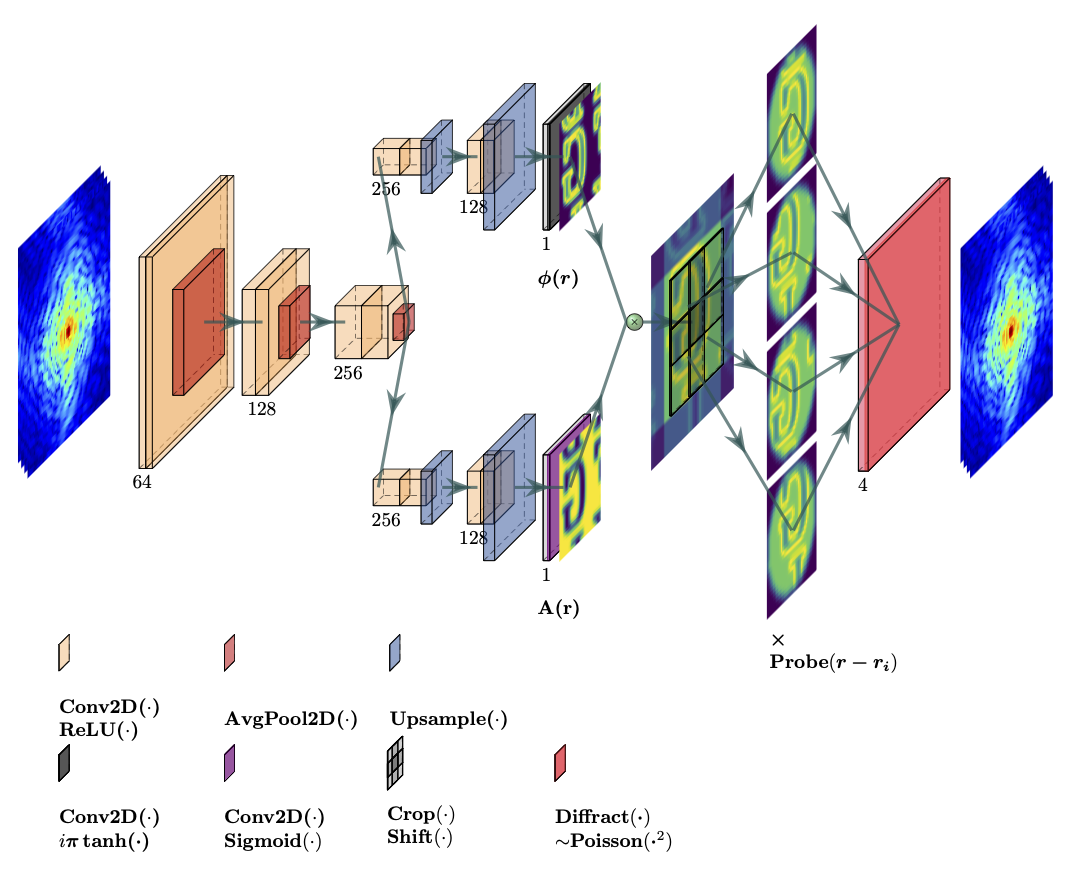
\includegraphics[width=0.9\textwidth]{figures/lett.png}
\caption{Neural network architecture and training configuration of the PtychoPINN model.}\label{diagram}
\end{figure}

\subsubsection{Map formulation}
The reconstruction problem requires approximating a mapping $G: X \rightarrow Y$ from the diffraction/reciprocal-space domain $X$ to the real-space domain $Y$. To do so without a need for labeled training data we rely on an autoencoder formalism that composes $G$ with a second mapping $F: Y \rightarrow X$, such that the autoencoder output is $\hat{x} = F(G(x))$, where $x$ is the (complex) diffracted wave field. \footnote{The measured diffraction intensity is therefore $I \appropto x^2 $.}.

In prior PINN approaches to CDI reconstruction, $F$ is typically the forward map of far-field diffraction. Here, we instead start by subdividing $F$ into two parts: a \emph{constraint} map $ F_c: Y \rightarrow Y$ and a diffraction map $ F_d: Y \rightarrow X$, such that $F(Y) = F_d(F_c(Y))$. The role of $F_c$ is to impose the real-space constraints necessary for exploiting overlapping diffraction measurements and making the inversion well posed. $F$ may depend on parameters $\theta$ such as the experimental geometry, so we relate it to a functional $\mathbf{F}$, such that $F = \mathbf{F}(\theta)$.

In our concrete implementation the elements of a set of training samples $\{x_i\}$ have shape $64 \times 64 \times 4$, corresponding to four diffraction patterns measured at neighboring scan point coordinates. We denote a particular diffraction image with index $k$ $(k \in \mathcal{K} = \{0, 1, 2, 3\}$) as $x_i^k$. Each $x_i$ is paired with its matching 2D Euclidean probe coordinates, $r_i$ ($r_i \in \theta$). Correspondingly, the reconstruction $y_i = G(x_i)$ is a 3D tensor of shape $32 \times 32 \times 4$. (The factor-of-two difference in size between $x_i$ and $y_i$ satifies the oversampling requirement for invertibility of the discrete Fourier transform \cite{miao2000oversampling}). Finally, to distinguish between the two real-space representations we let $\bar{y}_i = F_c(y_i)$. We denote the amplitude and phase of $\bar{y}$ as $A$ and $\phi$, respectively, throughout this paper.

The inverse map $G$ consists of an encoder-decoder architecture with a similar structure to PtychoNN and $F_d$ is mostly defined by diffraction physics. The element of most interest is $F_c$, which we detail below.
% TODO language



\subsubsection{Real-space constraints}
% TODO language, constraints etc.
%The phase problem in coherent diffractive imaging (CDI) reconstruction presents as invariant diffraction amplitudes due to real-space object inversion and translation. In the case of scanning CDI, it's necessary to solve this problem using real-space constraints that leverage overlapping measurements.
In CDI reconstruction the phase problem manifests as invariances of the diffraction amplitude to coordinate inversion and translation of the real-space object. In the case of scanning CDI this must be solved using real-space constraints based on overlapping measurements.

In order to detail how the real-space constraint map, $\mathbf{F_c}(r_i)$, is applied to $y_i$, we can break it down into two steps. Initially, we perform a summation of individual $y_i^k$ to create a unified reconstruction $\hat{y}_i$ with a shape of $64 \times 64$:
%
%We describe application of the real-space constraint map $\mathbf{F_c}(r_i)$ to $y_i$ in two steps. First, we sum the individual $y_i^k$ into a unified reconstruction $\hat{y}_i$ of shape $64 \times 64$:


\begin{equation} 
\hat{y}_i = \Sigma_{k \in \mathcal{K}} T(r_i^k - \mu_i, Pad2d(y_i^k))
\oslash
\Sigma_{k \in \mathcal{K}} T(r_i^k - \mu_i, Pad2d(\bf{1})), 
\label{eq:1}
\end{equation}

where $Pad2d$ denotes zero-padding a $32 \times 32$ tensor to $64 \times 64$ and $T(\delta r, y)$ is the translation of a 2D tensor $y$ by the vector $\delta r$. $\mu_i$ is the origin of a local coordinate system for the group of scan points and is normally set to their centroid position, for convenience. $\oslash$ represents elementwise division, while $\bf{1}$ stands for a $32 \times 32$ tensor composed entirely of ones. Therefore, the divisor $\Sigma_{k \in \mathcal{K}} T(r_i^k - \mu_i, Pad2d(\bf{1}))$ has the role of a normalizing tensor.

The purpose of this first transformation is to construct a larger real-space image $\hat{y}_i$ that encompasses the entire solution region. The second, and arguably more critical, step implements translational symmetry of the reconstruction, factoring in shifts in the probe location. This step also transforms the 2D object $\hat{y}_i$ into a 3D object that matches the downstream \textcolor{red}{lang?} shape of the autoencoder output $x_i$, and suits application of $F_d$:

$$
\bar{y}_i^k = T(\mu_i - r_i^k, \hat{y}_i) P(r) \approx O(r) P(r - r_i^k),\label{eq:2}
$$

Here, $O(r)$ represents the ground-truth object, with its (right hand side) discrete approximation domain confined to a $32 \times 32$ patch centered at $r_i^k$.

\textcolor{red}{transition?}

We can compare this approach to iterative scanning CDI reconstruction schemes, which enforce real-space constraints in a different way. In methods such as ePIE, the optimization loop is organized around alternating error corrections in real and reciprocal space. In the `backpropagation' step of ePIE, the error in diffraction reconstruction amplitude for one diffraction measurement -- equivalent to our our formulation's $\lvert x_i^k \rvert - \lvert \hat{x}_i^k \rvert $ -- induces an update of the $O(r)$ reconstruction via inverse DFT. In the training of PtychoPINN, errors from the $\vert \mathcal{K} \vert$ individual patterns are converted into model parameter updates instead of reconstruction updates, and this is done in parallel instead of sequentially.

\textcolor{red}{In the context of this paper $\vert \mathcal{K} \vert$ = 4 always and there's no need to assign a variable to the set of scan point coordinates, but the model supports other solution grid sizes (i.e., K =  4 x 4, 6 x 6, etc.). the parallelism benefit of processing 4 patterns at a time is small, but at 16 and beyond it might start to matter. this should make PtychoPINN faster than the baseline NN method, but this is probably stuff for another paper.}

%This formulation sets up unsupervised training using the diffraction forward map and additional constraints in real space. 
%With $\mathbf{F_c}(r_i)$ thus defined, we are now ready to apply the far-field diffraction map to each channel of $\bar{y}$.
% and the inverse DFT -- which is implicit in gradient calculation -- is performed 
%, and adjacent $x_i$..... \cite{epie} Our approach instead forces averaging directly in $Y$-space, which avoids the need for expensive back-and-forth transforms. \emph{delta y, within one forward pass, etc.}


%This approach leverages both the advantages of physics-based methods and the efficiency of neural networks, making it a powerful tool for CDI reconstruction.



\subsubsection{Probabilistic output and loss function}
%\subsubsection{Loss function}

%The model loss is a simple MAE objective over reconstructed diffraction 
%
%$$
%Loss(\hat{x}, x) = \sum_{i,j,k}\log f_{\text{Poiss}}(I_{ijk};\lambda_{ijk})
%$$

We choose the model output to be a collection of independent Poisson distributions parameterized by the forward-mapping of the final-layer output of the NN. This reproduces the correct photon-counting statistics of the diffraction measurement and allows us to calculate a likelihood, with respect to the Poisson parameters, for the distribution of per-pixel detected photon counts. The negative log over these Poisson likelihoods is \emph{a priori} a more principled loss function than the typical choice of mean absolute average (MAE) deviation between target and predicted pixel values.

Explicitly, the loss function is

$$
Loss(x, \lambda(\hat{x})) = \sum_{i,j,k}\log f_{\text{Poiss}}(x_{ijk}^2;\lambda_{ijk})
$$


where $\lambda_{ijk}(\hat{x}) = \hat{x}_{ijk}^2$, $x_{ijk}^2$ is the number of photons detected in a single pixel (its square root $x_{ijk}$ is the associated target amplitude), $\lambda_{ijk}$ is the matching final-layer output of the CNN, $i$ and $j$ index the detector coordinates, and $k$ indexes separate images within a diffraction set. 

For the above probabilistic formulation of the data, model output, and loss function to be self-consistent it is necessary for the units of the diffraction pixel values to be (unscaled) photon counts. A typical diffraction intensity is $10^9$ photons per exposure whereas the magnitude of activations within the NN -- including, in particular, the reconstructed real-space amplitude -- should be of order unity. To invertibly scale the input (and output) we define a global normalization parameter that we initialize using a simple heuristic based on the mean photon count of images in the training dataset and unitarity property of the Fourier transform.  (\textcolor{red}{ref appendix or supplemental materials for formula}). This normalization parameter can optionally be either fixed or optimized during training. 


\subsection{Data generation}\label{data}

\begin{figure}
    \centering
    {{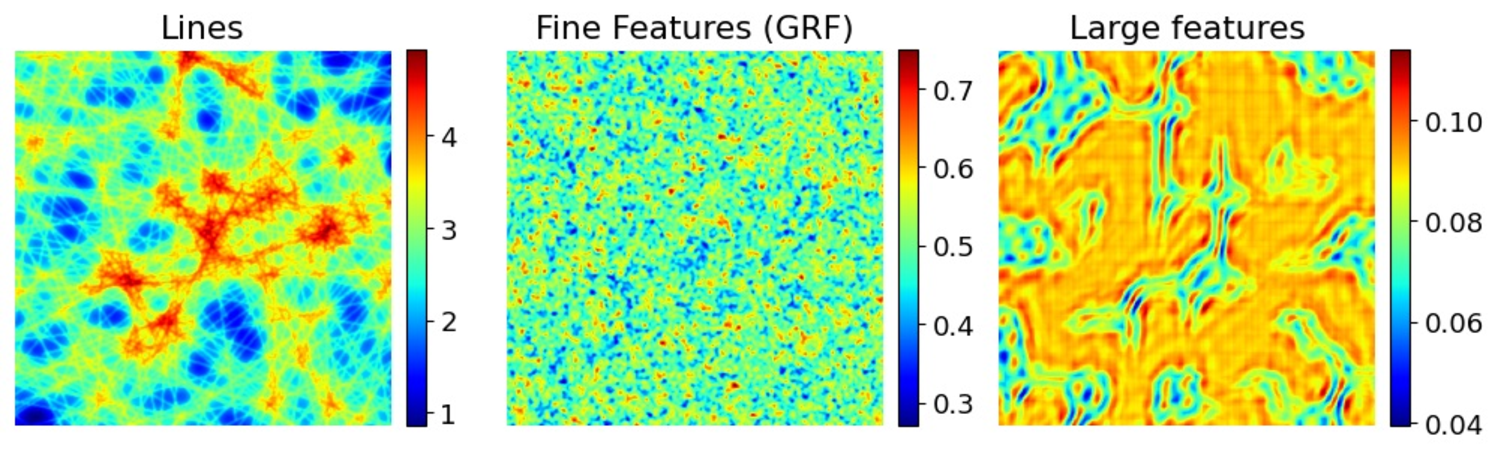
\includegraphics[width=12cm]{figures/datasets.png} }}%
    \caption{Representative samples from the three dataset types used in this investigation.}%
    \label{fig:datasets}%
\end{figure}

To prepare the model's training and evaluation data we begin with a collection of complex-valued images. We consider three types of images: simulated compositions of randomly-oriented lines, (simulated) Gaussian random field samples, and experimentally-derived phase and amplitude from x-ray ptychographic measurements of an etched tungsten test sample, which we retrieved from a publicly available dataset\cite{cherukara2020ai}. Representative samples of each dataset type are shown in Figure \ref{fig:datasets}, labeled respectively as Lines for randomly-oriented lines, GRF for Gaussian Random Field and Experimental for the Experimental data of \cite{cherukara2020ai}. For each real-space object dataset we simulate a collection of diffraction patterns corresponding to a rectangular grid of scan points on the sample and a known (complex-valued) probe function. Given the real-space object $O(r)$ and far-field diffraction forward map $F_d$, the simulated diffraction pixel values are random samples from $f_{\text{Poiss}}(F_d(O(r))^2)$, where $f_{\text{Poiss}}$ is the Poisson distribution.
% (for the ptychographic dataset, an ePIE reconstruction is used as ground truth)
% and $s$ is a dimensionless normalizing parameter that controls the average number of collected photons in the simulated diffraction. 


%First, we follow the proven approach of using an autoencoder formalism to reduce the problem to unsupervised training. We adopt a 2D covolutional architecture with one encoder to transform diffraction images into compact embeddings and two decoders to map those embeddings into real-space maps of phase and amplitude. The final stage of the model transforms the phase and amplitude into reciprocal-space complex object using the forward map of far field diffraction. \emph{cite PtychoNN, AutophaseNN}
%$F_d$ incorporates the far-field diffraction forward map and 
%(This grouping of neighboring measurements in the channel dimension is a requirement of the constraint map, which we will explain shortly.)
%; the purpose of $\mathbf{F_c}$ is to enforce those constraints. 

%To describe $\mathbf{F_c}$ we begin with the probe function $P(r)$, real-space object $O(r)$, and scan point coordinate $r_i^k$, which together define a complex-valued object $O_i^k(r) \equiv O(r) P(r - r_i^k)$. 
%
%$O_i^k(r)$ is the ground truth of a real-space image corresponding to a single diffraction measurement and $y_i^k = G(x_i)^k$ is a model estimate of $O_i^k(r)$. Instead of directly passing $y_i$ to the diffraction map we first apply the real-space transformation $\mathbf{F_c}(r_i)$. (Note the separation of $\mathbf{F(\theta) = \mathbf{F_c(\theta)} \circ \mathbf{F_d(\theta)}}$). 
%We separate $\mathbf{F_c}(r_i)$ into two steps. First, a summation of the individual $y_i^k$ into a unified reconstruction $\bar{y}_i$ of shape $64 \times 64$: 
%(The complex tensor $\bar{y}_i^k$ approximates an illuminated patch of the object.)
%TODO gradient spread between instances of the iteration loop

%The joining of ptychograpic overlap constraints with NN-based reconstruction is our framework's main contribution. \emph{belongs in intro, discussion or conclusions, but should be emphasized}
%, and numerical experiments can verify this expectation (\emph{ref Discussion section}).
%$$f_{\text{Poiss}}(k;\lambda) = e^{-\lambda} \frac{\lambda^k}{k!}$$

% Second, we make the ptychographic inversion well posed by imposing \emph{overlap} constraints in the reconstruction. In each forward pass the model processes a set of several diffraction patterns corresponding to overlapping illumination areas of the probe on the sample and maps that entire set of diffraction images into a single (average-reduced) complex-valued object. 

% Second, to make the ptychographic inversion well-posed we impose overlap constraints in the reconstruction process. Specifically, in each forward pass, our model processes a set of diffraction patterns that correspond to overlapping illumination areas of the probe on the sample. We then map this entire set of diffraction images into a single, complex-valued object by averaging overlapping regions. It is important to note that reconstructing a real-space object from an individual diffraction pattern is not possible due to the invariance of the Fourier Transform amplitude to coordinate inversion. As a result, each diffraction amplitude image corresponds to at least two real-space reconstruction candidates. This property is intentionally incorporated into our approach to make the Fourier Transform inversion well-posed, as in iterative algorithms such as ePIE. In ePIE, the backpropagation step of the iteration loop uses inverse-Fourier transformation to convert residuals on the reciprocal space amplitude of each individual diffraction pattern into incremental updates of a globally-shared estimate of the real-space object.

% In contrast to this overlap-merging setup, it is \emph{not} possible to reconstruct a real-space object from an individual diffraction pattern: the FT amplitude is invariant to coordinate inversion and therefore one diffraction amplitude image corresponds to at least two real-space reconstruction candidates (the inequality depends on whether additional degeneracies, such as translation invariance, are present). This is a deliberate adaptation of the property of iterative ptychographic reconstruction schemes that makes their FT inversion well-posed: in algorithms such as ePIE, one phase of the iteration loop -- the so-called backpropagation step -- uses inverse-Fourier transformation to convert residuals on the reciprocal space amplitude of each individual diffraction pattern into incremental updates of a globally-shared estimate of the real-space object. \emph{cite ePIE, etc.}
% This removes the inversion degeneracy that plagues PtychoNN.
% TODO amplitude map or complex object?


\subsection{Training}
%In each training instance, the dataset is a collection of simulated diffraction measurements derived from randomly-generated images, optical photographs, or experimental (x-ray ptychographic) images  \cite{cherukara2020ai}. 
%For the generated or photographic images, each training dataset contains 49,284 diffraction patterns densely sampleed from 9 simulated objects. The experimental dataset is limited to a single object with 16,100 corresponding diffraction patterns. 
For the non-experimental images, each training dataset contains 49,284 diffraction patterns densely sampled from 9 simulated objects. The experimental dataset is limited to a single object with 16,100 corresponding diffraction patterns. 

To train the model parameters we use the Adaptive Moment Estimation (ADAM) optimizer with an initial learning rate of 0.001.\cite{kingma2014adam} We train for 50 epochs and with a batch size of 16, which takes approximately 10 minutes on an Nvidia RTX 3090 GPU.

 % to adjust the model's parameters. At the end of each epoch, the model's performance is assessed using validation data. 
%The ReduceLROnPlateau callback is applied to decrease the learning rate by a factor of 2 when the NLL validation loss plateaus.


% TODO do we want full comparison of all the PINN variations here, or save that for the discussion section?

\section{Results and Discussion}

\subsection{Numerical experiments}


\begin{figure}%
    \centering
    \subfloat[\centering Ground truth $\phi$]{{\includegraphics[width=4cm]{figures/lines/gt_phi_lines4.png} }}%
    \subfloat[\centering PtychoNN $\phi$]{{\includegraphics[width=4cm]{figures/lines/PtychoNN_phi_lines4.png} }}%
    \subfloat[\centering PtychoPINN $\phi$]{{\includegraphics[width=4cm]{figures/lines/PtychoPINN_phi_lines4.png} }}%
\vfill
    \subfloat[\centering Ground truth $A$]{{\includegraphics[width=4cm]{figures/lines/ground_truth_lines4.png} }}%
    \subfloat[\centering PtychoNN $A$]{{\includegraphics[width=4cm]{figures/lines/ptychoNN_lines4.png} }}%
    \subfloat[\centering PtychoPINN $A$]{{\includegraphics[width=4cm]{figures/lines/PINN_lines4.png} }}%
    \caption{Reconstruction comparison, simulated data}%
    \label{fig:sim_comparison}%
\end{figure}

\begin{table}[h]
\begin{center}
\caption{Three reconstruction metrics for the baseline NN reconstruction model and several variations of the PINN architecture, repeated for three contrasting datasets (lines, GRF and experimental). The metrics are mean absolute error (MAE), peak signal to noise (PSNR), and the 50 percent threshold of the Fourier Ring Correlation (FRC50). }\label{tab1}%
\begin{tabular}{p{2cm}l|ll|ll|ll}
\toprule 
    %Model features & \multicolumn{1}{c}{} & \multicolumn{2}{c}{lines} & \multicolumn{2}{c}{GRF} & \multicolumn{2}{c}{experimental}\\
    & \multicolumn{1}{c}{} & \multicolumn{2}{c}{experimental} & \multicolumn{2}{c}{GRF} & \multicolumn{2}{c}{lines}\\
    \midrule
    &
    & $A$ & $\phi$
    & $A$ & $\phi$
    & $A$ & $\phi$ \\
    \midrule
$\{\}$\footnotemark[1]    
& MAE & 0.00394 & 0.542 & 0.0181 & 0.0458 & 0.0245 & 0.13 \\
& PSNR (db) & 92.9  & 50.6 & 80.9 & 71.9 & 40.4 & 62.8 \\
& FRC50 & 34 & 5 & 56 & 53 & 51 & 3 \\
    \midrule
$\mathrm{PINN} $
& MAE & 0.00598 & 0.495 & 0.0371 & 0.11 & 0.0386 & 0.164 \\
& PSNR (db) & 88.8  & 52.4 & 67 & 65.3 & 65 & 63.2 \\
& FRC50 & 8 & 8 & 26 & 6 & 25 & 11.5 \\
    \midrule
overlaps
& MAE & 0.00343 & 0.549 & 0.0166 & 0.0364 & 0.0269 & 0.187 \\
& PSNR (db) & 93.2  & 50.7 & \textbf{81.5} & 74.6 & 41 & 60.3 \\
& FRC50 & \textbf{39} & 1 & 62 & 6 & 49.5 & 2 \\
    \midrule
PINN,overlaps\footnotemark[2]    
& MAE & \textbf{0.00287} & \textbf{0.147} & \textbf{0.00543} & \textbf{0.012} & \textbf{0.00757} & \textbf{0.0208} \\
& PSNR (db) & \textbf{95.8}  & \textbf{61.1} & 80.5 & \textbf{84.5} & \textbf{60.9} & \textbf{79.7} \\
& FRC50 & \textbf{39} & \textbf{51} & \textbf{94} & \textbf{94} & \textbf{170} & \textbf{173} \\
\end{tabular}
\end{center}
\footnotetext[1]{supervised baseline}
\footnotetext[2]{full PtychoPINN}
\end{table}

\begin{table}[h]
\begin{center}
\caption{Numerical study of out-of-sample robustness corresponding to the data of Figure \ref{fig:gen_detailed}.}\label{tab2}%
\begin{tabular}{lcccc}
\toprule
           &      &      &  PSNR &  FRC50 \\
& Dataset & &       &        \\
\midrule
\multirow{4}{*}{PtychoPINN} & \multirow{2}{*}{train} & $A$ & 78.41 & 160 \\
           &      & $\phi$ & 69.11 & 158 \\
\cline{2-5}
           & \multirow{2}{*}{test} & $A$ & 61.11 &  42 \\
           &      & $\phi$ & 59.87 &  41 \\
\cline{1-5}
\cline{2-5}
\multirow{4}{*}{baseline} & \multirow{2}{*}{train} & $A$ & 73.72 &  76 \\
           &      & $\phi$ & 72.11 &  74 \\
\cline{2-5}
           & \multirow{2}{*}{test} & $A$ & 57.91 &  22 \\
           &      & $\phi$ & 55.77 &  18 \\
\bottomrule
\end{tabular}
\end{center}
\end{table}

Figure \ref{fig:sim_comparison} presents a comparison of the reconstruction of artificially generated objects (from the `lines' data type of Fig. \ref{fig:datasets}) using PtychoPINN and the supervised learning baseline, PtychoNN. In these reconstructions, PtychoPINN demonstrates little noticeable degradation in the real-space amplitude and phase. In contrast, the supervised learning baseline shows substantial blurring. The 50 percent threshold of the amplitude Fourier ring correlation (FRC50), a useful measure of linear resolution, is $50~\mathrm{pixel}^{-1}$ for the baseline and a considerably improved $170~\mathrm{pixel}^{-1}$ for PtychoPINN. Furthermore, the peak signal-to-noise ratio (PSNR), a standard metric for reconstruction quality in the super-resolution literature, is 10.3 dB higher for PtychoPINN. 

In order to explore the performance of the model across diverse data, we extended the evaluation to include two additional object types: those derived from Gaussian random field (GRF) generated objects and experimental measurements (Table \ref{tab1}). For the GRF dataset, improvements in both PSNR and FRC50 were relatively modest compared to the improvements seen in the line dataset. It should be noted, however, that the GRF dataset has a smaller dynamic range and inherently lacks sharp features, which simplifies the reconstruction task.

Fig. \ref{fig:exp_comparison_detailed}, we see that both PtychoPINN and PtychoNN yield good amplitude reconstructions of the experimental object. Yet, the baseline's satisfactory amplitude reconstruction stands in contrast to its more limited recovery of the phase image (FRC50 of $51~\mathrm{pixel}^{-1}$ and $5~\mathrm{pixel}^{-1}$, respectively for PtychoPINN and baseline). While both methods have some difficulty reconstructing the phase in areas of the object with low scattering amplitude, PtychoPINN proves more robust; the baseline model, on the other hand, has a propensity to incorrectly invert the phase in these low-amplitude regions (Fig. \ref{fig:exp_comparison_detailed}(b)).


\begin{figure}%
    \centering
    \subfloat[\centering Ground truth $\phi$]{{\includegraphics[width=4cm]{figures/gt_phi_experimental.png} }}%
    \subfloat[\centering PtychoNN $\phi$]{{\includegraphics[width=4cm]{figures/PtychoNN_phi_experimental.png} }}%
    \subfloat[\centering PtychoPINN $\phi$]{{\includegraphics[width=4cm]{figures/PtychoPINN_phi_experimental.png} }}%
\vfill
    \subfloat[\centering Ground truth $A$]{{\includegraphics[width=4cm]{figures/ground_truth_experimental.png} }}%
    \subfloat[\centering PtychoNN $A$]{{\includegraphics[width=4cm]{figures/ptychoNN_experimental.png} }}%
    \subfloat[\centering PtychoPINN $A$]{{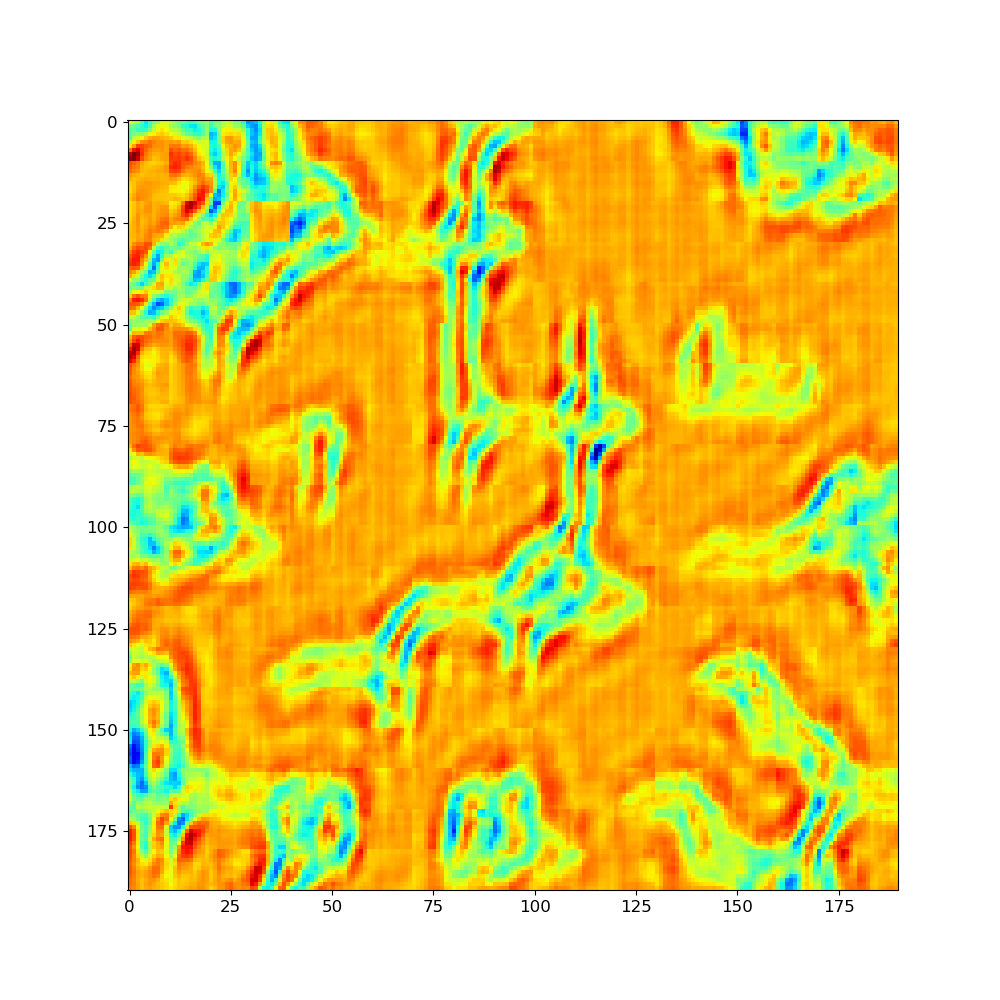
\includegraphics[width=4cm]{figures/PINN_experimental.png} }}%
    \caption{Reconstruction comparison, experimentally-derived data}%
    \label{fig:exp_comparison_detailed}%
\end{figure}

\subsubsection{Ablation study}
%To better understand the specific aspects of PtychoPINN that contribute to its improved performance, we conducted an ablation study evaluating the impact of unsupervised/PINN-based training, real-space constraints, and the choice of loss function (diffraction MAE vs. Poisson NLL). The comparison of reconstruction mean absolute errors (MAEs) in Table \ref{tab1} suggests that the combination of overlap constraints and PINN structure is the most significant factor in improving performance. It is worth noting that neither the PINN architecture nor the overlap constraints yield a substantial improvement in reconstruction accuracy when used separately. Moreover, we observed a small but consistent improvement in performance when using the Poisson NLL objective.

To better understand the specific aspects of PtychoPINN that contribute to its improved performance, we conducted an ablation study evaluating the impact of PINN-based training and real-space constraints. The comparison of reconstruction accuracy (MAE), resolution (Fourier ring correlation, FRC), and peak signal-to-noise ratio (PSNR) in Table \ref{tab1} suggests that the combination of overlap constraints and PINN structure is the most significant factor in improving performance. (\emph{Combination} is an important qualifier, as neither the PINN architecture nor the overlap constraints yields a substantial improvement in reconstruction accuracy when used individually.)
% TODO language, elaborate

\subsubsection{Out-of-sample generalization}
To complement these standard evaluation metrics we tested PtychoPINN's out-of-sample generalization. For this purpose, we extracted two distinct $392 \times 392$ patches from a larger image and used just one patch for training both the PtychoPINN model and the baseline model (Figure \ref{fig:gen_detailed}).

In order to provide a rigorous test of the models' out-of-sample performance, we intentionally selected two image patches with considerable divergence in their features. This choice of markedly different images creates a more stringent test of out-of-sample behavior than the other datasets that we have presented.

By comparing the models' reconstructions of the first (in-sample) and second (out-of-sample) patches, we can make a qualitative assessment of their respective out-of-sample generalization capabilities. As depicted in Fig. \ref{fig:gen_detailed}, the comparison of panels (c) and (f) (representing PtychoPINN) to panels (b) and (e) (representing the baseline model) demonstrates a significantly smaller out-of-sample deterioration in reconstruction quality for PtychoPINN, which suggests that our proposed model exhibits improved generalization ability compared to the baseline. The respective numerical comparison (Table \ref{tab2}) supports this assertion, displaying a smaller drop in PSNR between the training and out-of-sample data for PtychoPINN. However, it should be noted that both PtychoPINN and the baseline experience a roughly two-fold reduction in FRC50.
%By examining each model's reconstruction of the first (in-sample) and second (out-of-sample) patches we can qualitatively judge the two models' out-of-sample generalization. The comparison of Fig. \ref{fig:gen_detailed} (c) and (f) (ours) to Fig. \ref{fig:gen_detailed} (b) and (e) (baseline) shows a much smaller out-of-sample degradation in reconstruction quality for PtychoPINN. 


% a composition of lines by PtychoNN, a basic PINN, and PtychoPINN, with all three models trained on the same GRF dataset. While the basic PINN and PtychoPINN both recover recognizable line features, PtychoNN produces objects that are quasi-reproductions of the GRF morphology, with no recovery of details smaller than the probe dimension. 

\subsection{Discussion}
We have presented PtychoPINN, an unsupervised learning approach for scanning coherent diffraction imaging (CDI) that integrates real-space constraints with a physics-informed neural network (PINN) architecture. This framework yields substantial improvements in reconstruction accuracy and resolution while preserving the inherent speed of NN-based reconstruction. 

%\emph{outline of transition paragraph}
%\begin{itemize}
%\item The main purpose of this transition is to introduce the notion that we're going to present a perspective of the model that emphasizes model properties that a domain scientist looking to put the model to practical use would be interested in. 
%\item For each of these properties, we will also try to understand \emph{why} the model has that property, from the point of an ML person interested in the underlying mechanics. 
%\item The properties are: unsupervised trainning, generalization,  and resolution / accuracy.
%\end{itemize}

In the ensuing discussion, our primary objective is to shed light on the features of our model that would be most intriguing to a domain scientist intending to deploy the model in practical applications. Simultaneously, we aim to decipher \emph{why} our model exhibits these characteristics, adopting the perspective of a machine learning investigator with an interest in the underlying mechanics. We specifically concentrate on three essential attributes: unsupervised training, generalization, and the interplay between resolution and accuracy.

\subsubsection{Unsupervised training} 
Unsupervised training provides numerous advantages over supervised learning methods. Key benefits include the ease of gathering training data and the capability to conduct model updates on the fly. The resulting ability to train on a corpus of training samples drawn from a similar distribution as the test-time samples curtails the risks of any problems in out-of-distribution generalization that a model might suffer from. 

 These advantages are particularly valuable in real-time experimental settings.

\subsubsection{Generalisation} \label{sec_generalization}

\begin{figure}%
    \centering
    \subfloat[\centering Ground truth]{{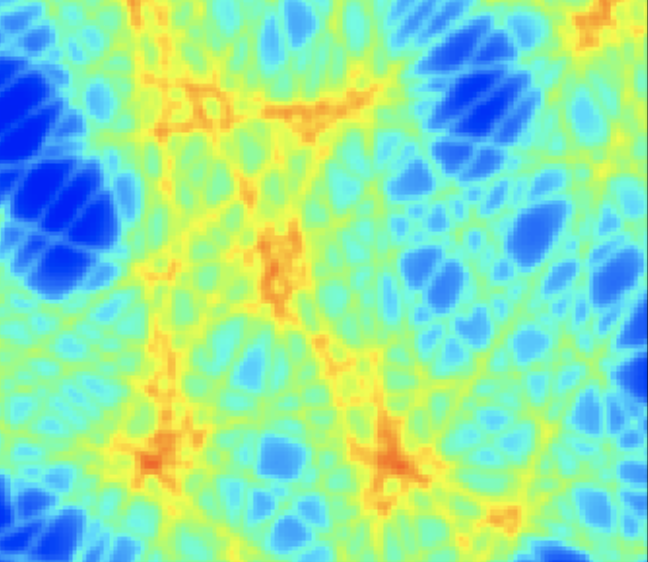
\includegraphics[width=4cm]{figures/generalizability_gt.png} }}%
    \subfloat[\centering PtychoNN]{{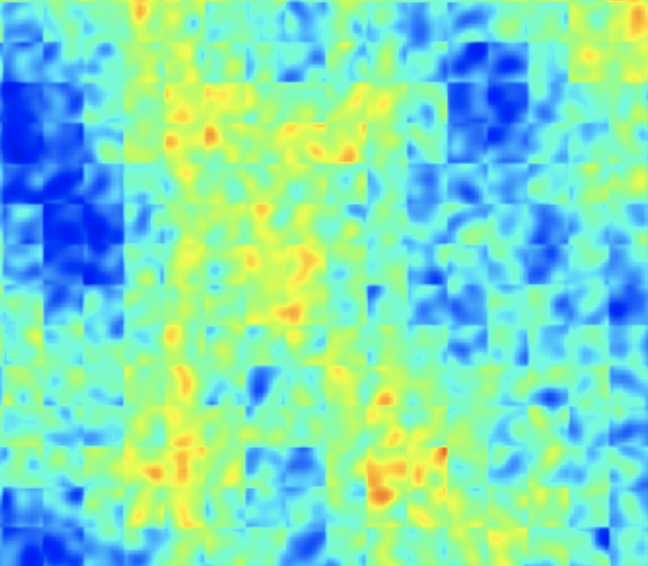
\includegraphics[width=4cm]{figures/generalizability_PtychoNN.png} }}%
    \subfloat[\centering PINN]{{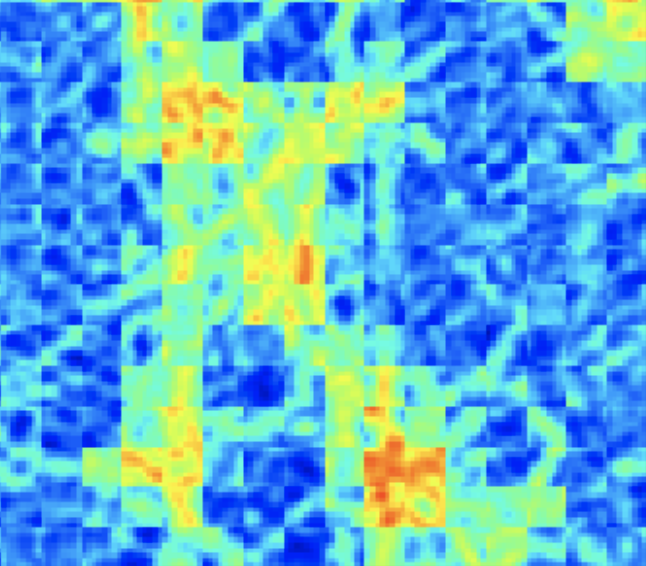
\includegraphics[width=4cm]{figures/generalizability_PINN.png} }}%
    \caption{Comparison of the simplified PINN (without overlap constraints) and PtychoPINN, both trained on Gaussian random field (GRF) objects and tested on compositions of lines......}
\label{fig:gen}%
\end{figure}

% Moreover, our numerical experiments demonstrate what we believe to be an inherent advantage of PINN architectures: improved generalization. We find that the basic PINN without overlap constraints displays superior out-of-sample generalization compared to the standard supervised learning approach (Figure \ref{fig:gen}).

% We attribute this improved generalization to the PINN structure. The structure requires the inverse map $G(X)$ to learn diffraction physics, facilitated by its connection to the far-field diffraction map $F_d$ and diffraction-space loss function $L$. This connection ensures a level of physical consistency between the real-space reconstruction and the measured diffraction. In contrast, supervised training often leads to breaches of even coarse conservation laws, such as the unitarity of the Fourier Transform.



%\subsubsection{Generalization}

\begin{figure}%
    \centering
    \subfloat[\centering Ground truth, training]{{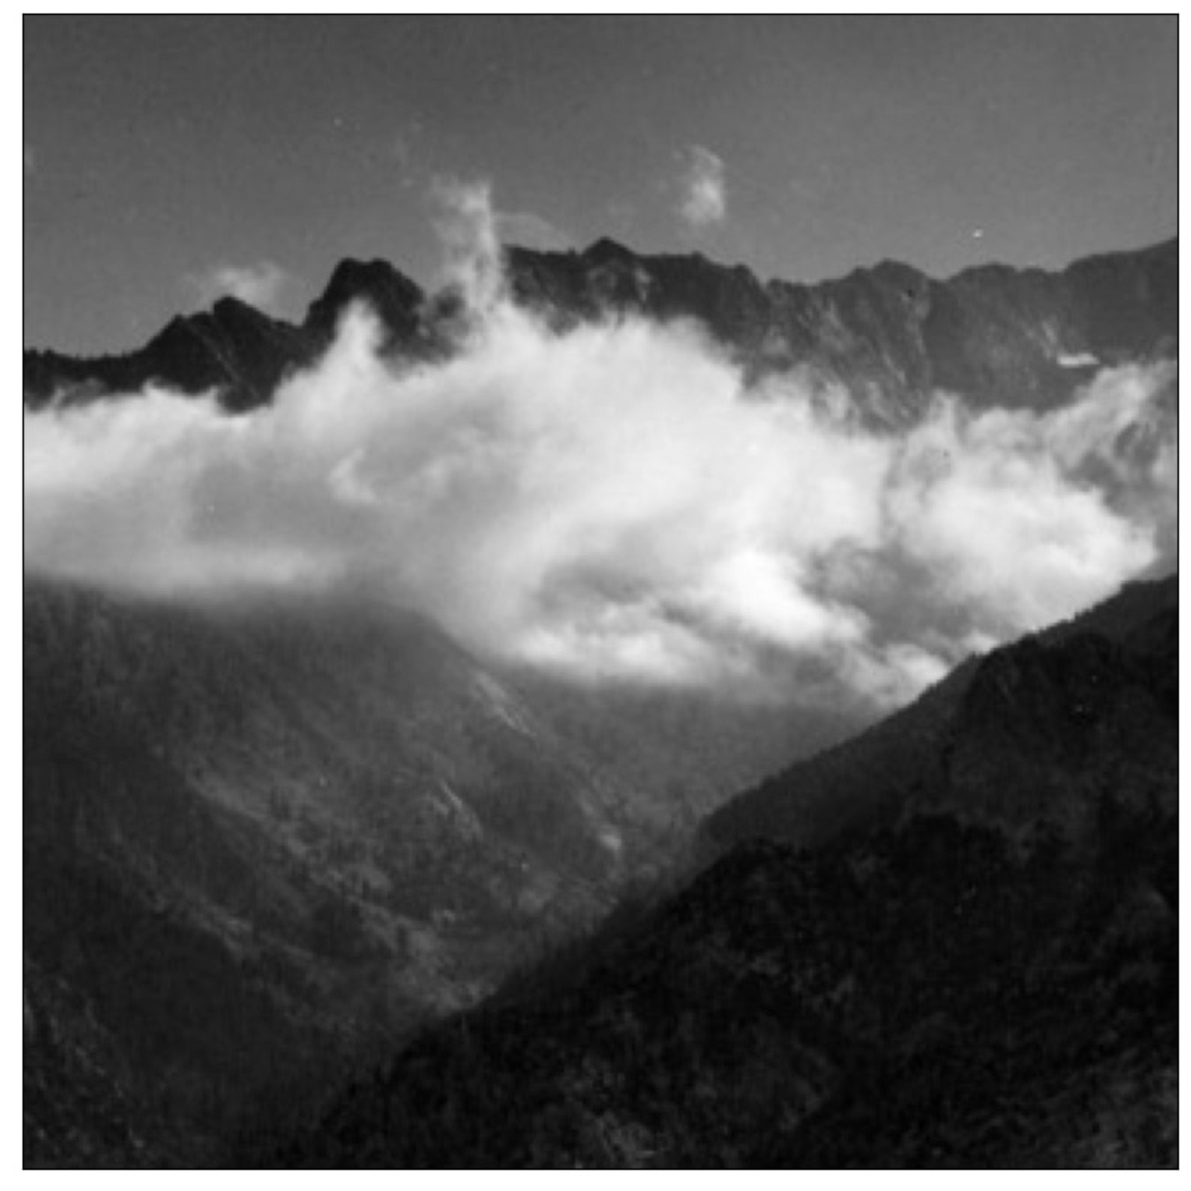
\includegraphics[width=4cm]{figures/generalization/gen_gt_train.png} }}%
    \subfloat[\centering baseline, in-sample ]{{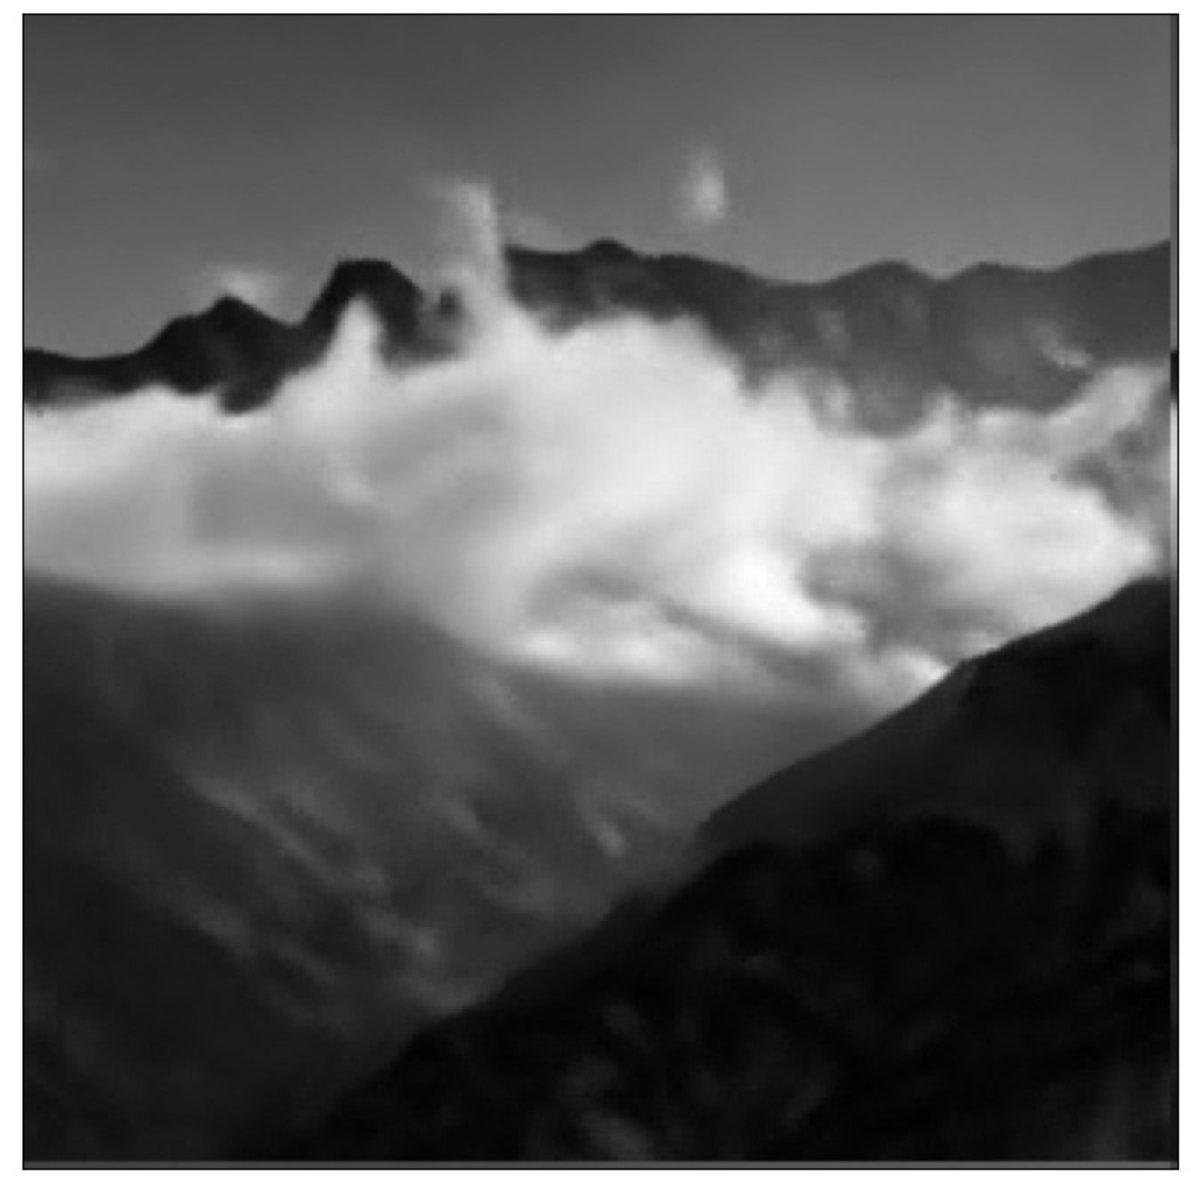
\includegraphics[width=4cm]{figures/generalization/gen_ptychoNN_train.png} }}%
    \subfloat[\centering ours, in-sample]{{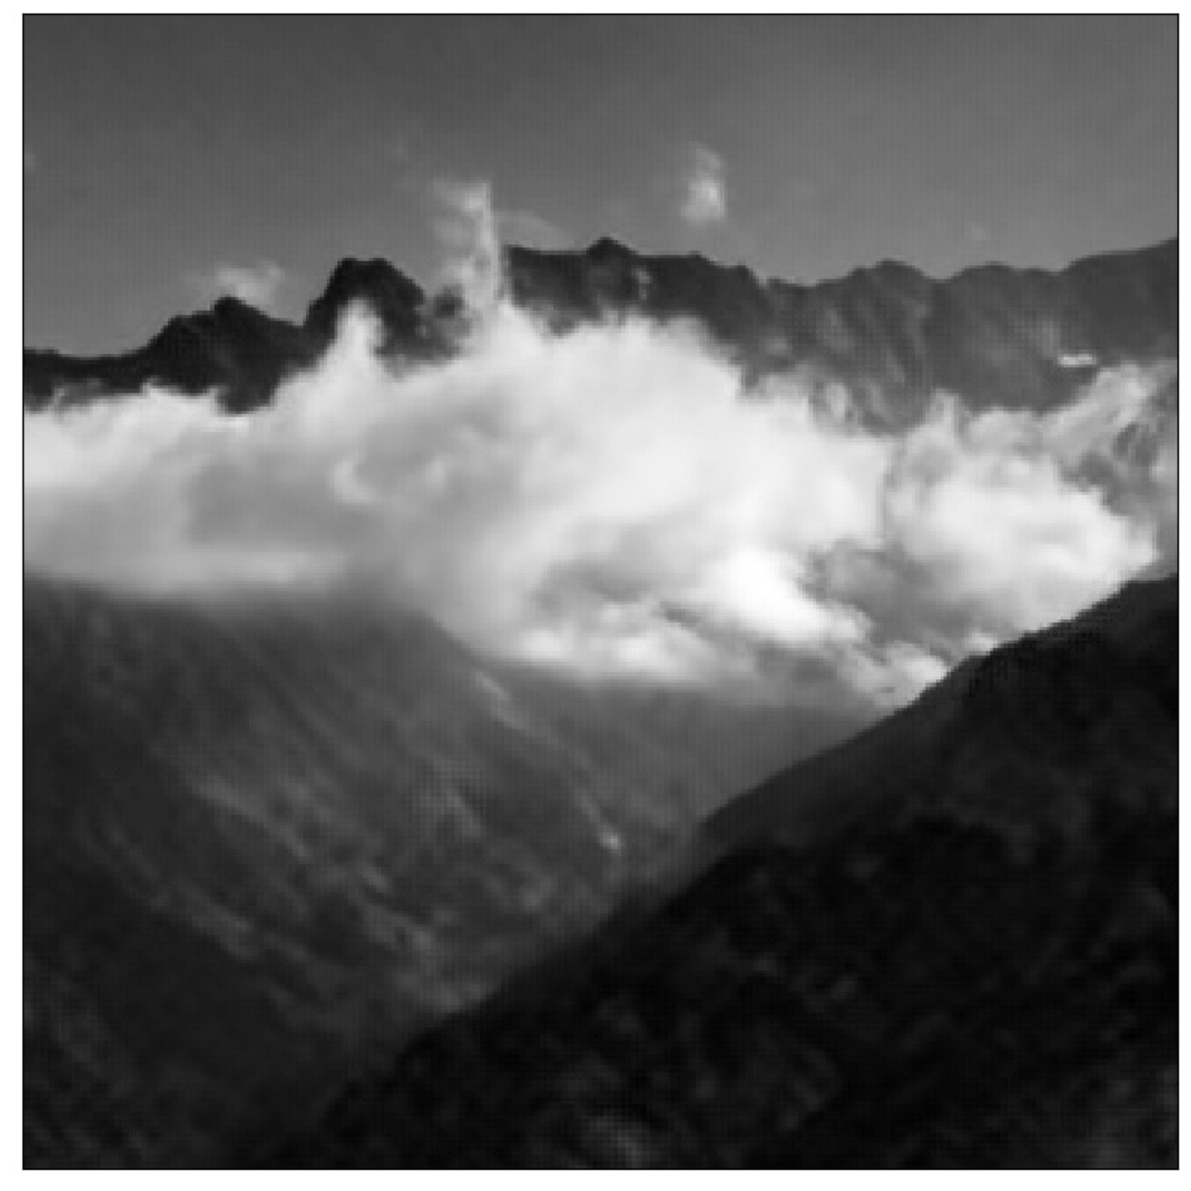
\includegraphics[width=4cm]{figures/generalization/gen_ptychoPINN_train.png} }}%
\vfill
    \subfloat[\centering Ground truth, out-of-sample]{{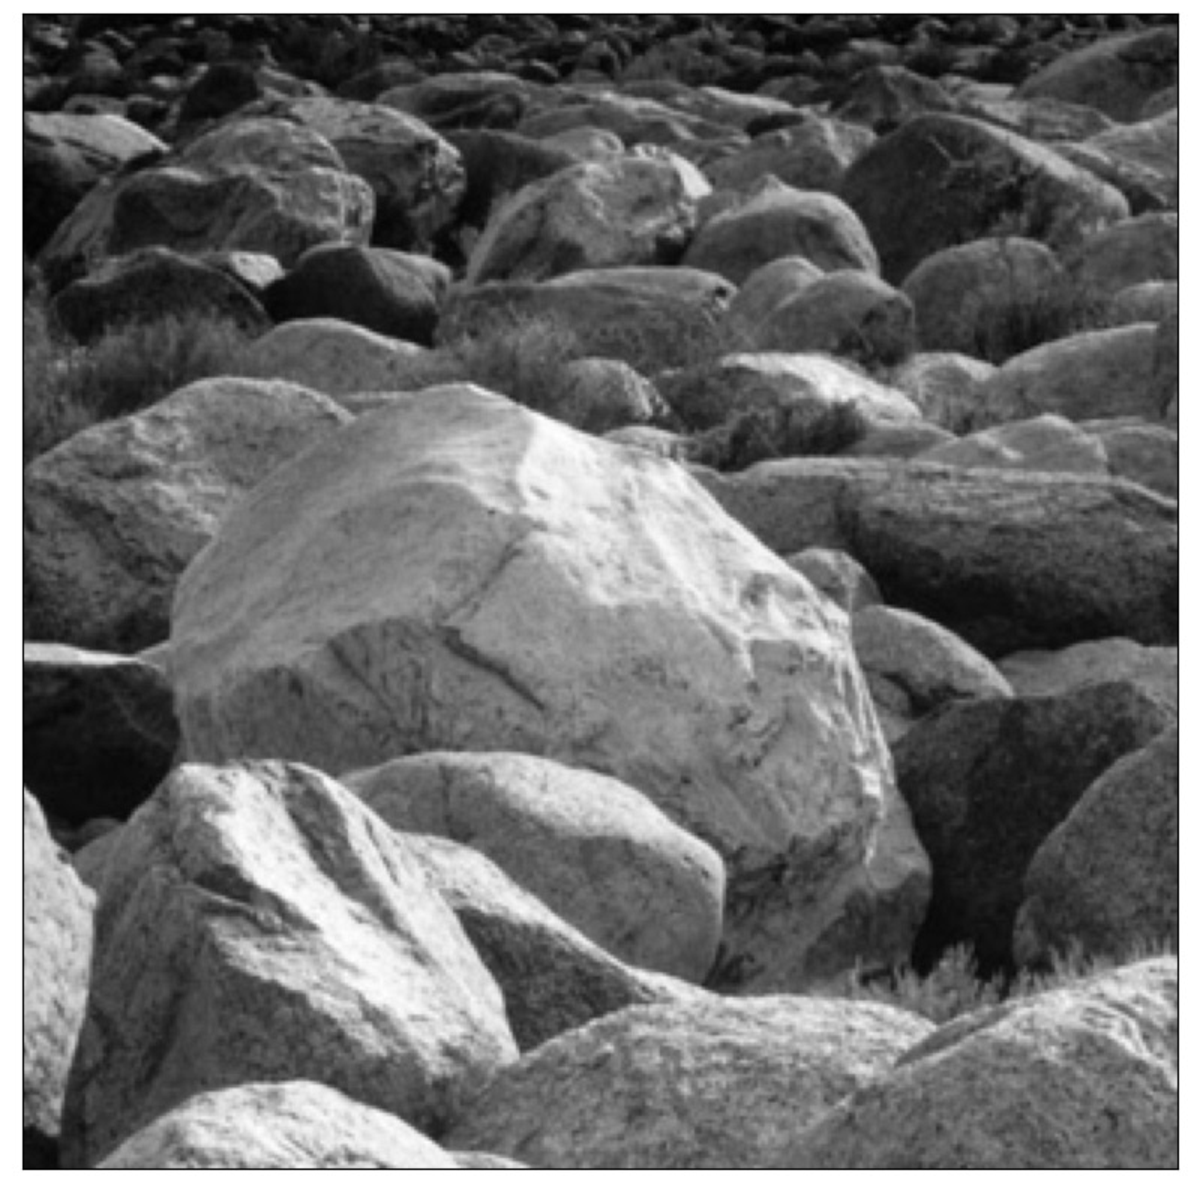
\includegraphics[width=4cm]{figures/generalization/gen_gt_test.png} }}%
    \subfloat[\centering baseline, out-of-sample]{{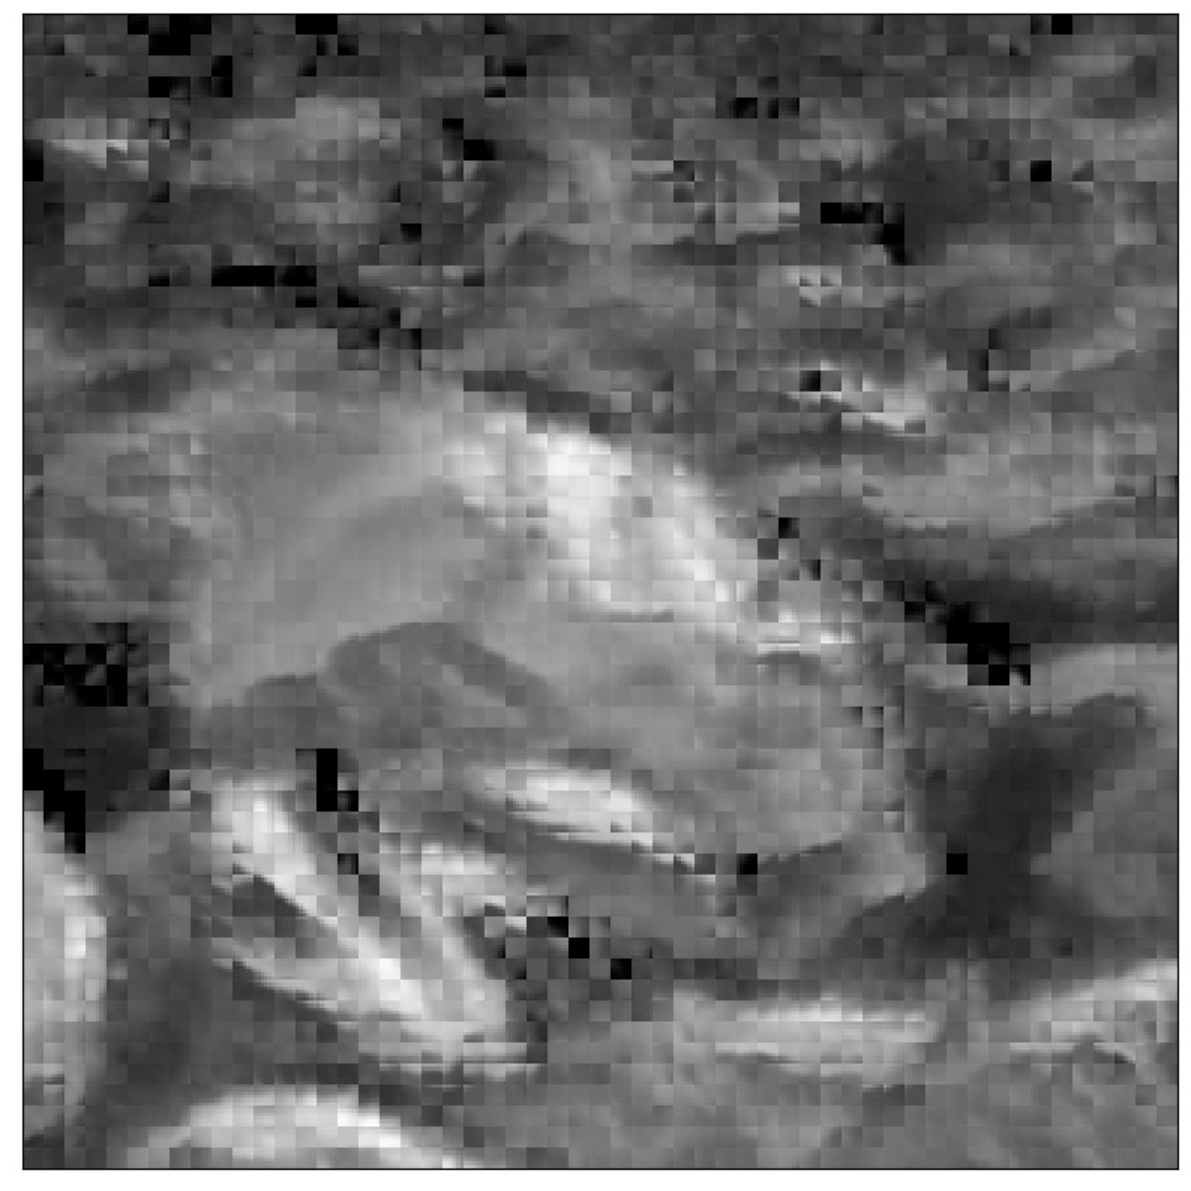
\includegraphics[width=4cm]{figures/generalization/gen_ptychoNN_test.png} }}%
    \subfloat[\centering ours, out-of-sample]{{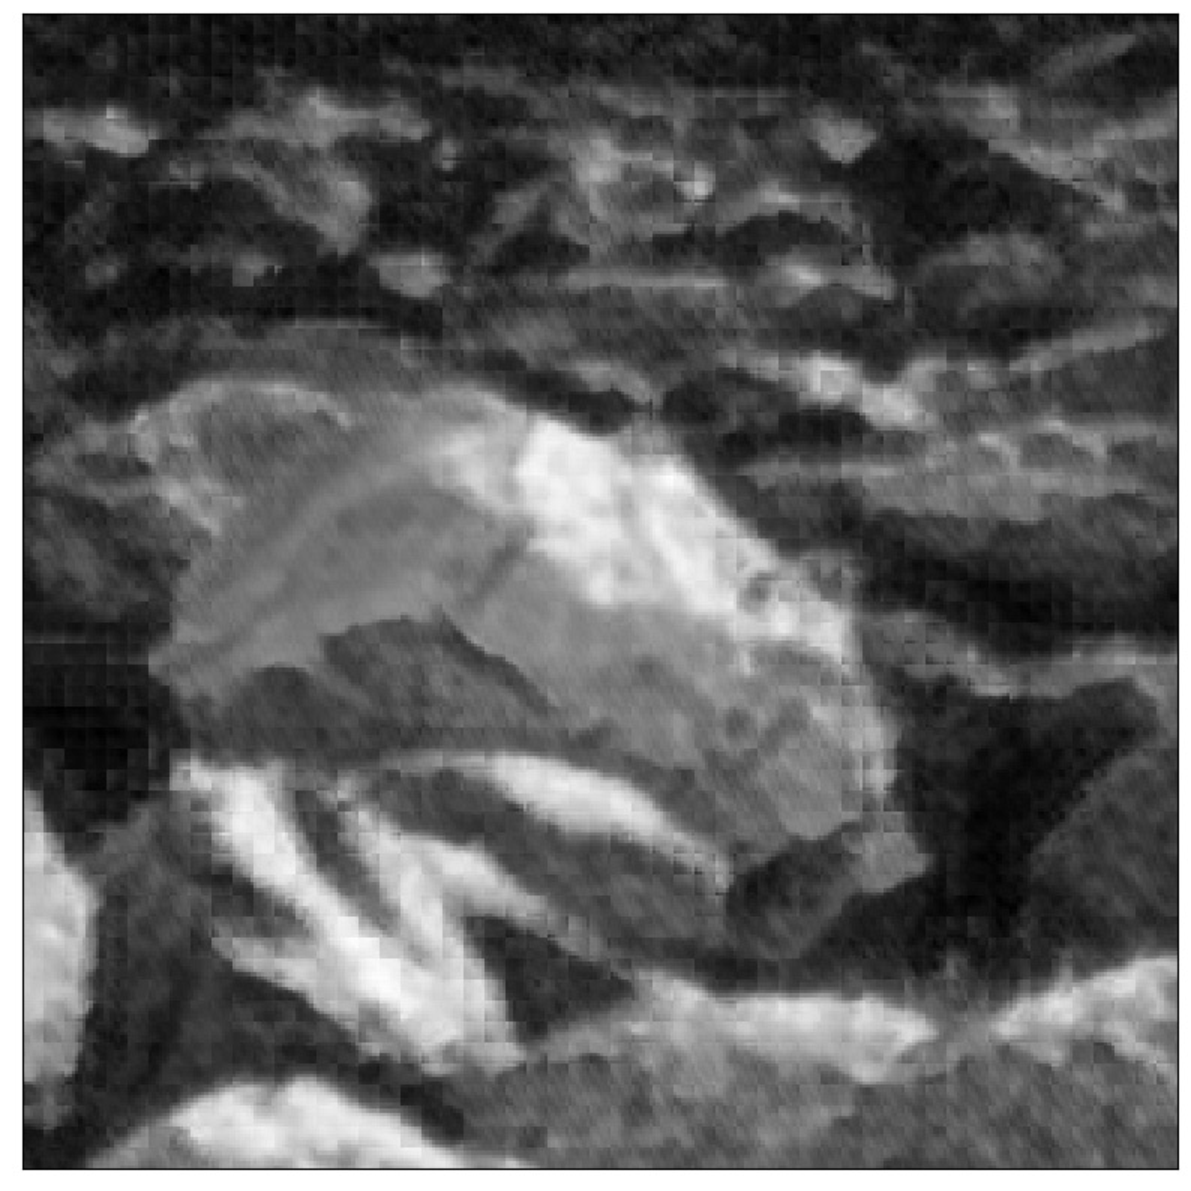
\includegraphics[width=4cm]{figures/generalization/gen_ptychoPINN_test.png} }}%
    \caption{Generalisation comparison between PtychoPINN and baseline (PtychoNN). Both models are trained on data derived from amplitude object (a). The trained models then reconstruct both the training image ((b) and (c)) and an out-of-sample image ((e) and (f)). All images are of real-space amplitudes; associated phase objects are not shown.  }%
    \label{fig:gen_detailed}%
\end{figure}


Additionally, we find that the PINN architecture possesses another inherent advantage: superior generalization. Even a simple PINN without overlap constraints demonstrates better out-of-sample generalization compared to the baseline supervised learning approach (Figure \ref{fig:gen}). 
\textcolor{red}{sentence here on the second generalization study, fig. \ref{fig:gen_detailed}}
We attribute this to the PINN structure, which necessitates the inverse map $G(X)$ to learn diffraction physics through its connection to the far-field diffraction map $F_d$ and diffraction-space loss function $L$. This association enforces approximate physical consistency between the real-space reconstruction and the measured diffraction. In contrast, supervised training in practice leads to violations of even coarse conservation rules, such as the FT's unitarity (i.e., $\lVert x \rVert \approx \lVert F_c(G(x)) \rVert = \lVert F_d(\bar{y}) \rVert = \lVert \hat{x} \rVert$, by Parseval's identity and $\bar{y} \equiv F_c(G(x))$).


Moreover, since $\hat{x} = F_d(\bar{y})$ is not a bijection and the loss function does not directly depend on $\bar{y}$, the PINN structure inherently disregards differences in real-space structure that are undetectable in the diffraction measurement. Conversely, supervised training is susceptible to wasting model capacity by memorizing the training data's real-space structure. All told, supervised learning approaches face challenges in generalization due to the difficult task of reconstructing an \emph{a priori} arbitrary map $X \rightarrow \hat{Y}$ with less guidance by useful inductive biases.

\subsubsection{Resolution and Accuracy}

\begin{figure}
    \centering
    \subfloat[\centering ]{{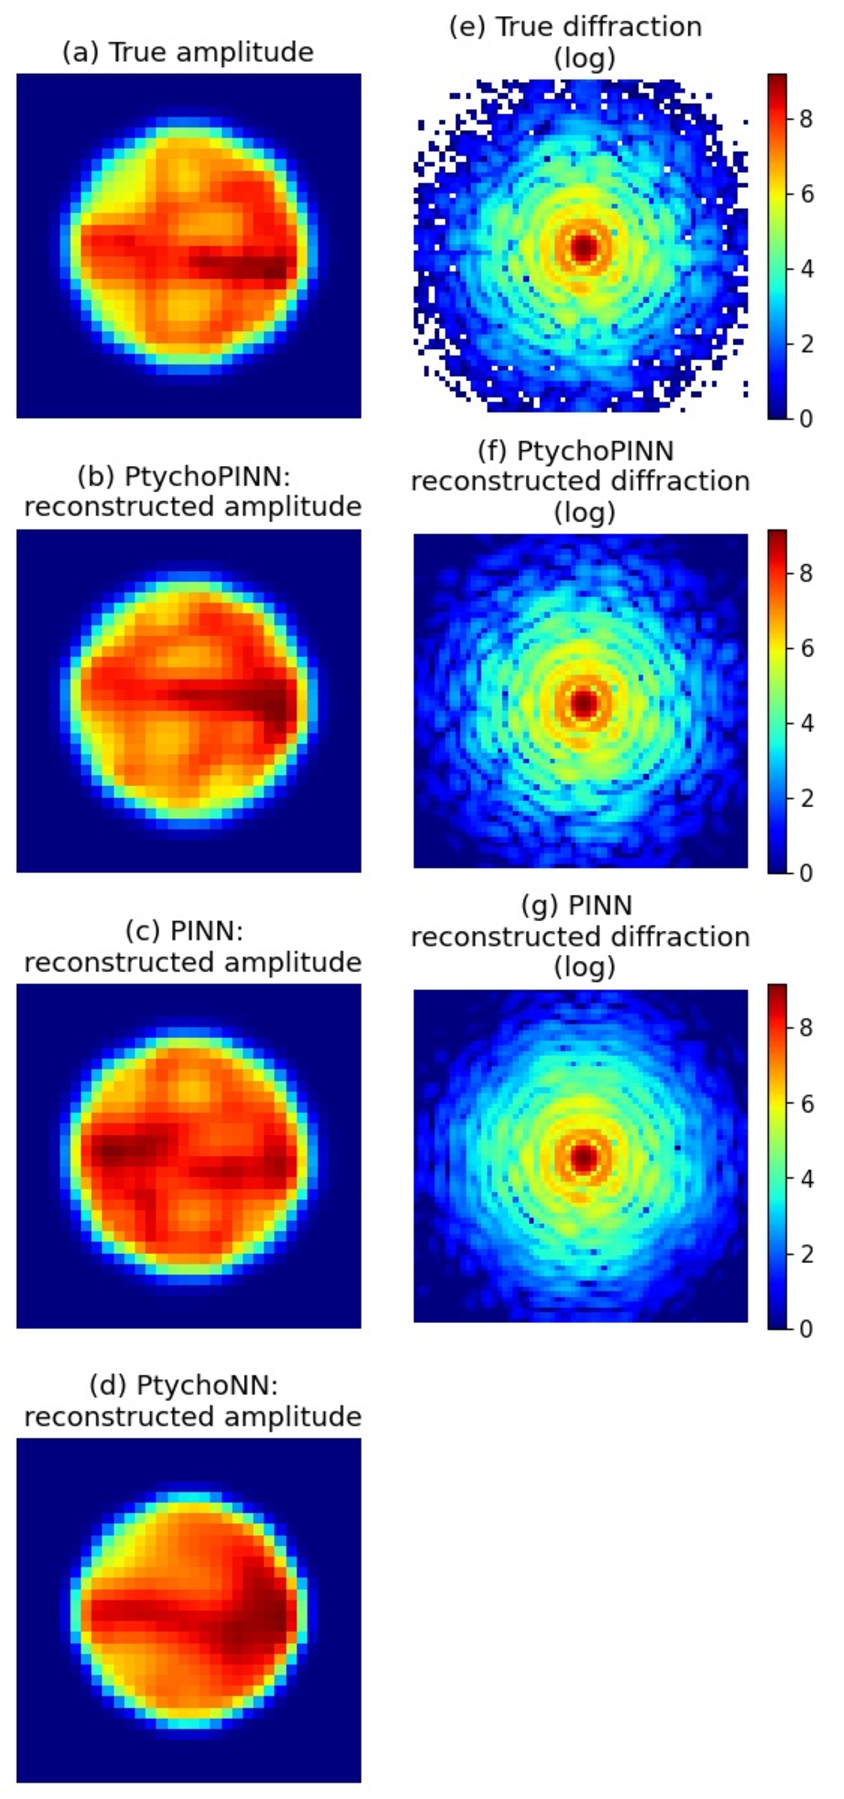
\includegraphics[width=12cm]{figures/patches.png} }}%
    \caption{Comparison of real-space and diffraction reconstructions from PtychoPINN and the simple PINN with no overlap constraints.}%
    \label{fig:patches}
\end{figure}

The advances in reconstruction quality presented by PtychoPINN hold two-fold significance: they bear practical implications for scientific applications, and also offer potential insights into the workings of the model itself. To facilitate a more nuanced understanding of the model, we distinguish between the concepts of \emph{resolution} and \emph{accuracy}.

Resolution, while a critical component of good reconstruction, is not alone sufficient. By comparing $32 \times 32$ reconstruction patches from PtychoPINN, PtychoNN, and a basic PINN (Figure \ref{fig:patches}), we observe that the basic PINN's reconstruction of line features displays a sharpness on par with PtychoPINN's. However, in contrast to both PtychoNN and PtychoPINN, the basic PINN misplaces these features. This arises due to the far field diffraction forward map's invariance to coordinate inversion, meaning real-space objects $O(r)$ and $O(-r)$ yield identical diffraction amplitudes. Thus, the basic PINN fails to distinguish between reconstruction pairs that are mirror images, or chiral, to each other.
\footnote{It might be worthwhile to make a distinction between local resolution - resolution within a single solution region - and the overall resolution in an image that has been composed from multiple reconstruction patches. The term 'resolution', as used in this context, specifically refers to the former.
% \textcolor{red}{Add something about the distinction between local resolution (in a single solution region) and resolution in an entire image stitched together from individual reconstruction patches. The usage of  `resolution' in this section only works for the former}

Local resolution pertains to the detail and sharpness within individual reconstruction patches, while global resolution refers to the reconstruction of features across the entire stitched-together image. The latter requires correct $O(r) / O(-r)$ parity within individual reconstruction patches, a more stringent condition.}

This PINN structure undoubtedly contributes a substantial enhancement to resolution, but it doesn't correspondingly boost \emph{accuracy}. In contrast, the inclusion of real-space overlap constraints in PtychoPINN overcomes the degeneracy linked with pairs of coordinate inversion-equivalent candidate objects. This leads to PtychoPINN's large enhancement in the accuracy of reconstruction -- however, it's worth emphasizing that this improvement primarily results from the correct alignment of high-spatial frequency features, and not from an increase in the amount of underlying image information.


% Discussion, old version
%In this work we introduced PtychoPINN, an unsupervised learning approach for scanning CDI that marries real-space constraints with a physics-informed neural network (PINN) architecture. The result is a framework that combines near-order of magnitude improvements in reconstruction accuracy and resolution with the intrinsic speed of NN-based reconstruction. 
%
%The unsupervised training of such Physics-Informed Neural Network (PINN) based approaches is an immediate benefit over supervised learning methods: it greatly increases the available amount of training data, reduces dependence on out-of-sample generalization, and facilitates on-the-fly model updates -- all important advantages for real-time scientific uses.
%
%Moreover, and less immediately obvious, we find a second intrinsic strength of PINN architectures: superior generalization. Specifically, even a rudimentary PINN without overlap constraints yields better out-of-sample generalization compared to the baseline supervised learning approach (Figure XX, supplemental materials). This may be because the PINN structure requires the inverse map $G(X)$ to conform to diffraction physics via its coupling to the far field diffraction map $F_d$ and diffraction-space loss-function $L$. This pairing imposes $\lVert x \rVert \approx \lVert F_c(G(x)) \rVert = \lVert F_d(\bar{y}) \rVert =  \lVert \hat{x} \rVert$ (by FT norm-conservation and the definition $\bar{y} \equiv F_c(G(x))$). Further, the diffraction-space loss function automatically respects FT symmetries, which reduces the PINN's opportunity to waste model capacity on memorizing particular training sample geometries. In contrast, the supervised learning approach fits a mapping between reciprocal-space and real-space images without the guidance of any inductive biases, including important constraints such as the Fourier transform's unitarity. 
%
%PtychoPINN's progress in reconstruction quality is interesting from two points of view: first, in its practical importance to scientific uses; and second, as a means of interpreting the behavior of the model itself. It is useful here to make a distinction between \emph{resolution} and \emph{accuracy}. 
%
%Resolution is an aspect of reconstruction quality that is necessary for a good reconstruction but \emph{not} on its own sufficient. Comparison of $32 \times 32$ reconstruction patches from PtychoPINN, PtychoNN and a basic PINN (\emph{Fig. xx}, supplemental materials) reveals that the basic PINN's reconstruction of line features has comparable sharpness to PtychoPINN's but, unlike both PtychoNN and PtychoPINN, the basic PINN alters the placement of those features. Unambiguously, this is a consequence of the far field diffraction forward map's invariance to coordinate inversion: real-space objects $O(r)$ and $O(-r)$ produce identical diffraction amplitudes and therefore the basic PINN is unable to distinguish between pairs of reconstructions that are chiral images of one another. 
%
%We can thus see that the PINN structure brings a large improvement in resolution with no corresponding improvemnt in \emph{accuracy}. In PtychoPINN, the addition of real-space overlap constraints breaks the degeneracy associated with each pair of coordinate inversion-equivalent real-space candidates. PtychoPINN's gains in accuracy thus come from its correct placement of high-spatial frequency features-- not large gains in the underlying information content of the real-space reconstruction. 
%(Equivalently, recall our earlier note that the role of the constraint map $F_c$ is to solve the intrinsic ill-posedness of the CDI phase problem.)
%
%%and can be used to compare the quality of different methods. With PtychoPINN, the improvement in linear resolution ranges between 3x and 30x for contrasting sharp-featured images. This is a remarkable result, especially when considering that it is mainly a product of the PINN architecture. This can be seen from the vanilla PINN's reconstruction of significantly finer real-space features, which demonstrates the advantage of the PINN structure in improving resolution.


\section{Conclusion}
\begin{itemize}
\item Sketch out areas of future improvement / exploration. Position correction; regularization; probablistic approaches to develop calibrated uncertainty quantification and better robustness. \emph{Interpretability} will also be an interesting aspect to explore, as it could give insight into the underlying mechanics of the more surprising aspects of the behavior of this new model / class of models.
\end{itemize}
\textcolor{red}{add a discussion of directions for probabilistic modeling, exploring robustness benefits of the NLL loss}


%\section{Conclusion}\label{sec13}

%%=============================================%%
%% For presentation purpose, we have included  %%
%% \bigskip command. please ignore this.       %%
%%=============================================%%

%%=============================================%%
%% For presentation purpose, we have included  %%
%% \bigskip command. please ignore this.       %%
%%=============================================%%

%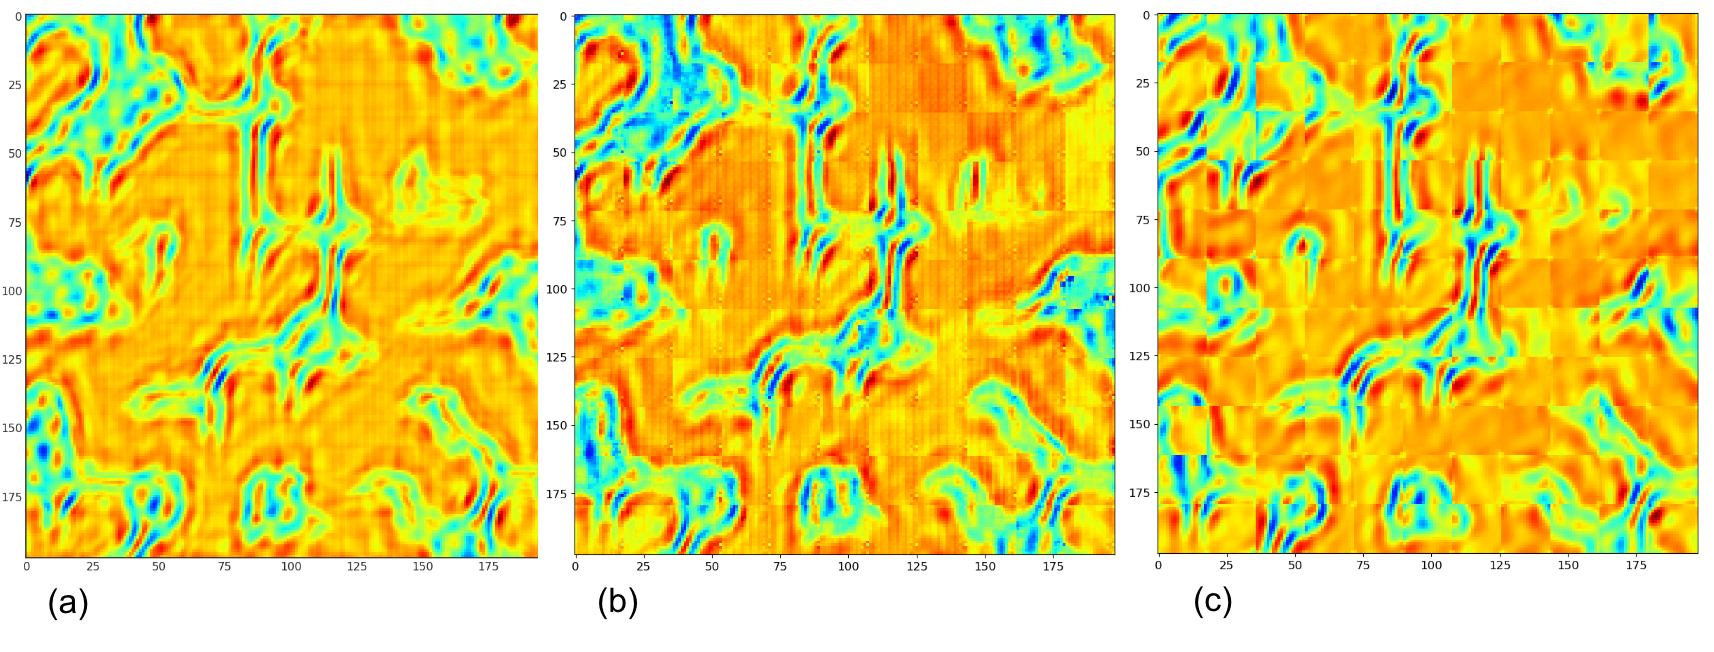
\includegraphics[width=0.9\textwidth]{figures/experimental.png}
%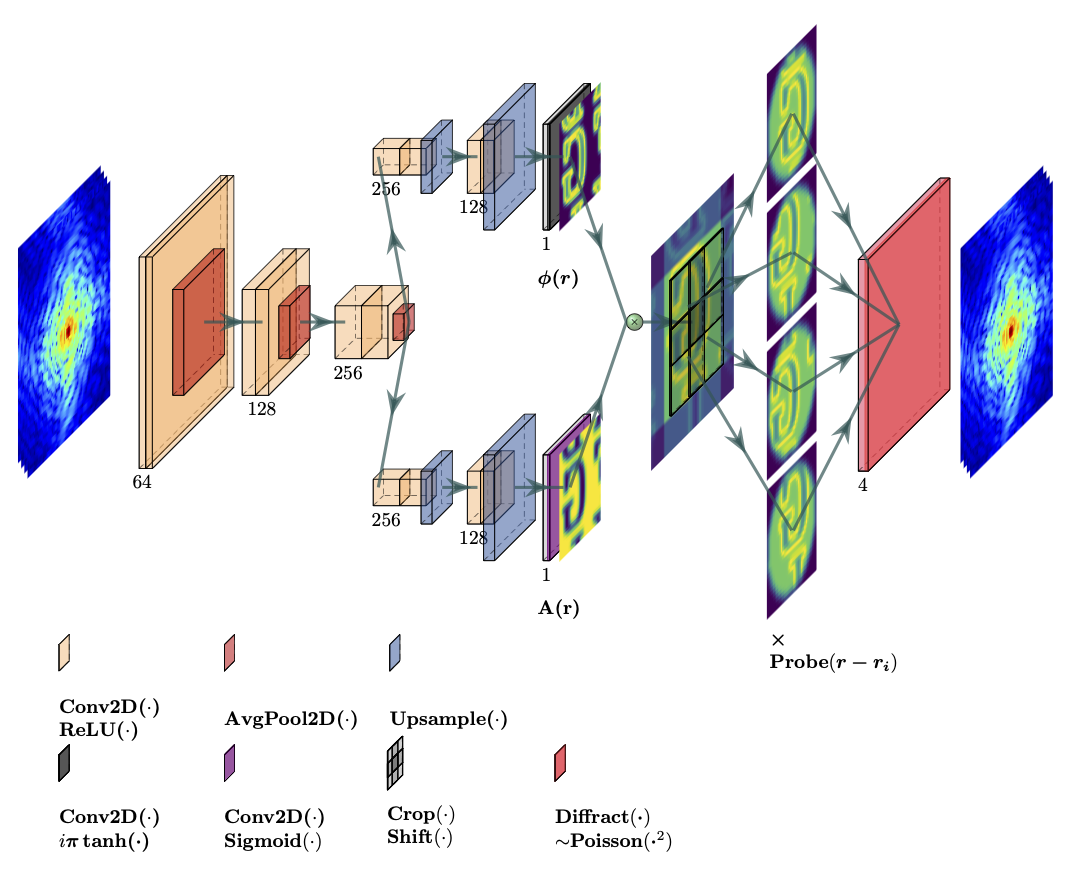
\includegraphics[width=0.9\textwidth]{figures/lett.png}




% \begin{figure}%
%     \centering
%     \subfloat[\centering Ground truth]{{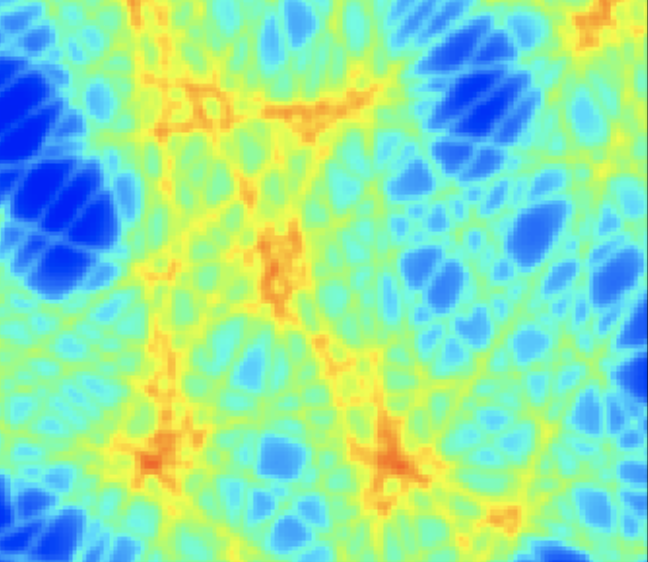
\includegraphics[width=4cm]{figures/generalizability_gt.png} }}%
%     \subfloat[\centering PtychoNN]{{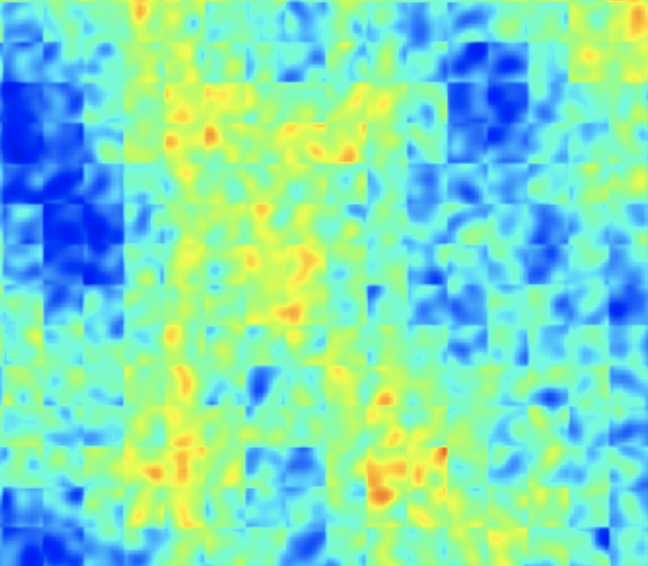
\includegraphics[width=4cm]{figures/generalizability_PtychoNN.png} }}%
%     \subfloat[\centering PINN]{{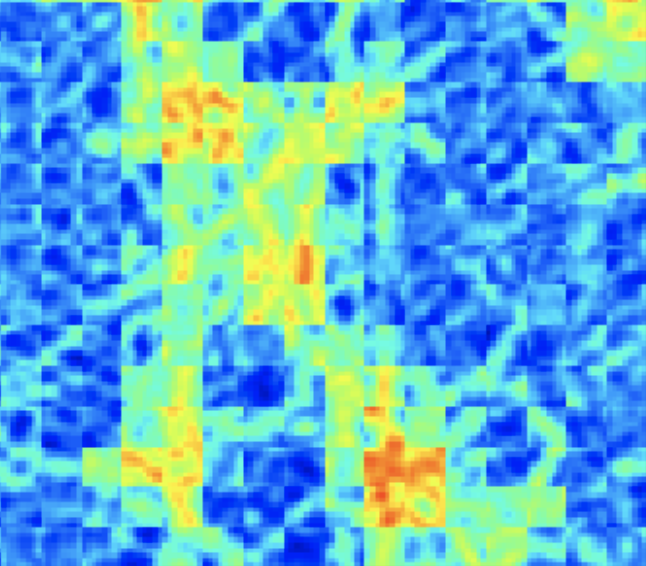
\includegraphics[width=4cm]{figures/generalizability_PINN.png} }}%
%     \caption{Test of generalizability}%
%     \label{fig:general}%
% \end{figure}







% \begin{figure}%
%     \centering
%     \subfloat[\centering Ground truth]{{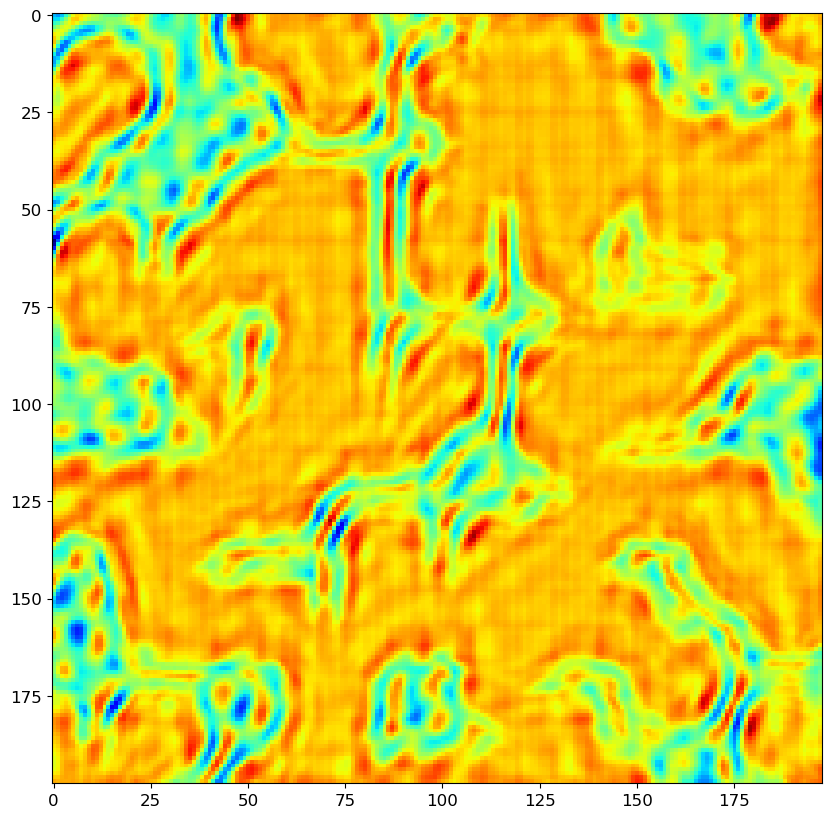
\includegraphics[width=4cm]{figures/gt_experimental.png} }}%
%     \subfloat[\centering PtychoNN]{{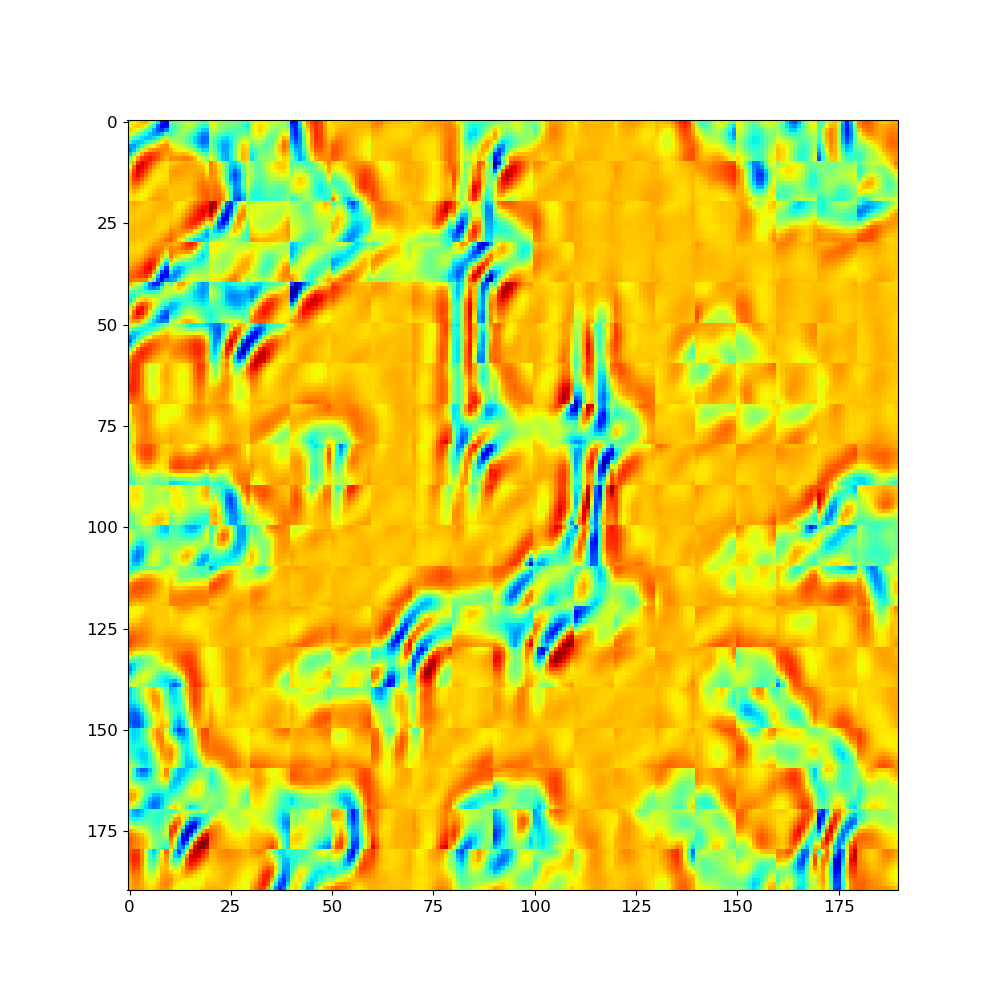
\includegraphics[width=4cm]{figures/PtychoNN_experimental.png} }}%
%     \subfloat[\centering PtychoPINN]{{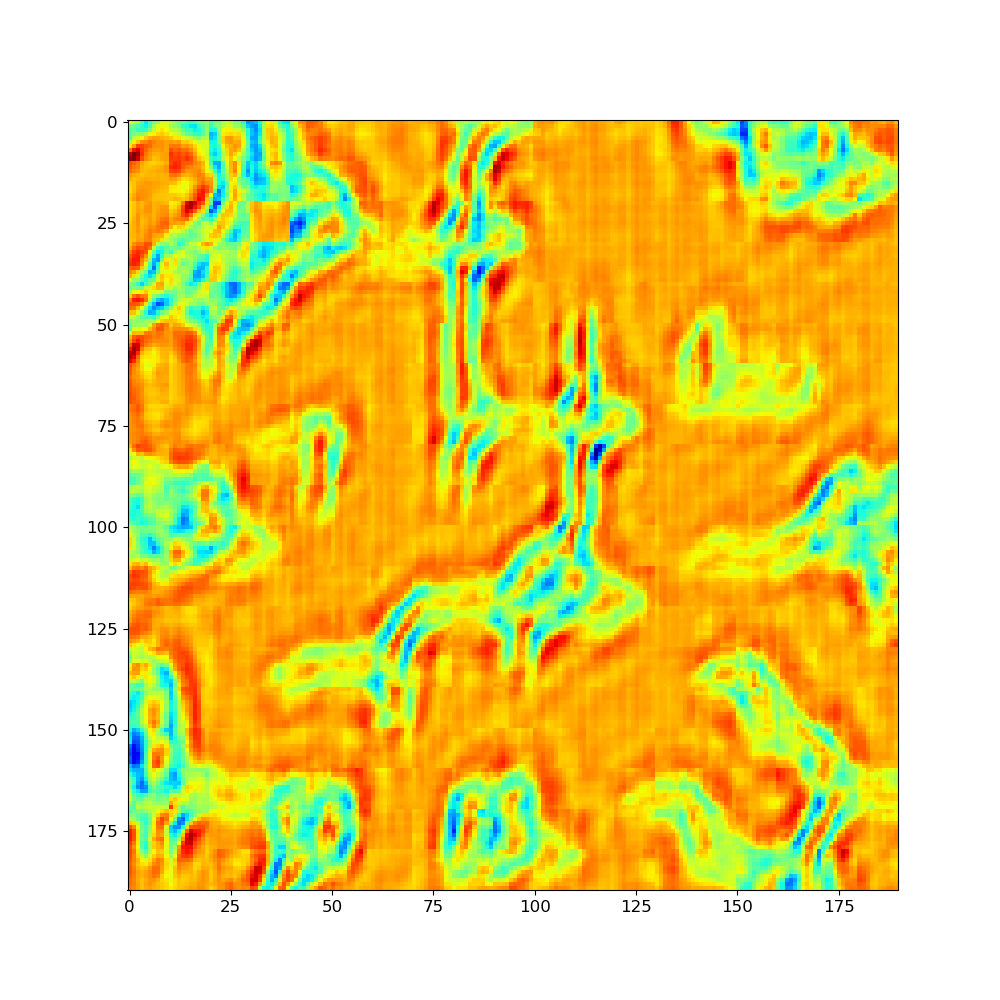
\includegraphics[width=4cm]{figures/PINN_experimental.png} }}%
%     \caption{Reconstruction comparison, experimental data. }%
%     \label{fig:exp_comparison}%
% \end{figure}



%\begin{table}[h]
%\begin{center}
%\caption{Three reconstruction metrics for the baseline NN reconstruction model and several variations of the PINN architecture, repeated for three contrasting datasets (lines, GRF and experimental). The metrics are mean absolute error (MAE), peak signal to noise (PSNR), and the 50 percent threshold of the Fourier ring correlation (FRC50) }\label{tab3}%
%\begin{tabular}{p{2cm}l|ll|ll|ll}
%\toprule 
%    & \multicolumn{1}{c}{} & \multicolumn{2}{c}{experimental} & \multicolumn{2}{c}{GRF} & \multicolumn{2}{c}{lines}\\
%    \midrule
%    &
%    & $A$ & $\phi$
%    & $A$ & $\phi$
%    & $A$ & $\phi$ \\
%    \midrule
%$\{\}$ \footnotemark[1]    
%& MAE & 0.00394 & 0.542 & 0.0181 & 0.0458 & 0.0245 & 0.13 \\
%& PSNR & \textbf{92.5} & 50.6 & 80.9 & 71.9 & 40.4 & 62.8 \\
%& FRC50 & 34 & 5 & 56 & 53 & 51 & 3 \\
%    \midrule
%$\{$overlaps$\}$
%& MAE & \textbf{0.00343} & \textbf{0.549} & \textbf{0.0166} & \textbf{0.0364} & 0.0269 & 0.187 \\
%& PSNR & 93.9 & 50.4 & \textbf{81.5} & \textbf{74.6} & 41 & 60.3 \\
%& FRC50 & 39 & 1 & 62 & 6 & 49.5 & 2 \\
%    \midrule
%$\{\mathrm{PINN}  \}$
%& MAE & 0.00598 & 0.495 & 0.0371 & 0.11 & 0.0386 & 0.164 \\
%& PSNR & 53.8 & 52 & 67 & 65.3 & 65 & 63.2 \\
%& FRC50 & 8 & 8 & 26 & 6 & 25 & 11.5 \\
%    \midrule
%$\{$PINN,~overlaps$\}$
%& MAE & \textbf{0.00287} & 0.147 & 0.00543 & 0.012 & \textbf{0.00757} & \textbf{0.0208} \\
%& PSNR & 54.8 & \textbf{60.8} & 80.5 & \textbf{84.5} & \textbf{60.9} & \textbf{79.7} \\
%& FRC50 & 39 & \textbf{51} & \textbf{94} & \textbf{94} & \textbf{170} & \textbf{173} \\
%    \bottomrule
%\end{tabular}
%\end{center


%In this table, we need 
%a) Additional datasets to test on (can be just one more, but needs to be different). To report the robustness of results.
%b) Do we have the variation about the mean? Was there significant variation due to the ordering of batches, initializations, etc in repeated experiments?
% a) is pretty much required.





\backmatter


\bmhead{Supplementary information}

\section*{Declarations}

\begin{itemize}
\item Funding
\end{itemize}


%%===================================================%%
%% For presentation purpose, we have included        %%
%% \bigskip command. please ignore this.             %%
%%===================================================%%
\bigskip


\begin{appendices}

\section*{Miscellaneous}
\begin{itemize}

\item The underlying manifold on which solutions live is smaller than the 64 x 64 output size ( oversampling requirement). Unsupervised models that are aware of this (e.g. AutophaseNN, PtychoPINN) thus have an output space of the correct (i.e. smaller) size. This may in part explain the PINN's better generalization / performance even in the absence of overlap information. We haven't mentioned this in the text, could go under Discussion / generalization.
\item cite ansel adams print \cite{adams1944mount}
\end{itemize}

% \begin{table}[h]
% \begin{center}
% \caption{Reconstruction accuracy (test MAE) for the baseline NN reconstruction model and several variations of the PINN architecture, repeated for three contrasting datasets. }\label{tab2}%
% \begin{tabular}{p{2cm}llllll}
% \toprule 
%     Model features & \multicolumn{2}{c}{lines} & \multicolumn{2}{c}{GRF} & \multicolumn{2}{c}{experimental}\\
%     & MAE($A$) & MAE($\phi$)
%     & MAE($A$) & MAE($\phi$)
%     & MAE($A$) \\%& MAE($\phi$) \\
%     \midrule
% $\{\}$ \footnotemark[1]    & 0.036   & 0.12  & 0.027 & 0.045 & 0.028 \\
% $\{\mathrm{PINN}  \}$  & 0.036   & 0.077 & 0.049 & 0.088 & 0.039 \\
% $\{$overlaps$\}$  & 0.025 & 0.19 &  0.020 & 0.033 & 0.027 \\
% $\{$PINN,~overlaps$\}$   & 0.0077 & 0.019 & 0.0077 & \bf{0.011} & 0.025 \\
%   $\{$PINN,~NLL$\}$     & 0.043    &   0.18  & 0.049 & 0.12 &  0.038 \\
%   $\{$PINN,~NLL,\newline
%  ~~overlaps$\}$     & \bf{0.0076}    &   \bf{0.014}  & \bf{0.0078} & .012 &  \bf{0.022}  \\
%     \bottomrule
% \end{tabular}
% \end{center}
% \footnotetext[1]{PtychoNN baseline}
% \end{table}

%%=============================================%%
%% For submissions to Nature Portfolio Journals %%
%% please use the heading ``Extended Data''.   %%
%%=============================================%%

%%=============================================================%%
%% Sample for another appendix section			       %%
%%=============================================================%%

%% \section{Example of another appendix section}\label{secA2}%
%% Appendices may be used for helpful, supporting or essential material that would otherwise 
%% clutter, break up or be distracting to the text. Appendices can consist of sections, figures, 
%% tables and equations etc.

\end{appendices}

%%===========================================================================================%%
%% If you are submitting to one of the Nature Portfolio journals, using the eJP submission   %%
%% system, please include the references within the manuscript file itself. You may do this  %%
%% by copying the reference list from your .bbl file, paste it into the main manuscript .tex %%
%% file, and delete the associated \verb+\bibliography+ commands.                            %%
%%===========================================================================================%%

\bibliography{ptycho-pinn}% common bib file
%% if required, the content of .bbl file can be included here once bbl is generated
%%\input sn-article.bbl

%% Default %%
%%\input sn-sample-bib.tex%

\end{document}
